\documentclass[12pt, letterpaper]{article}
\usepackage{bbold}
\usepackage{indentfirst}
\usepackage{amsmath, amssymb}
\usepackage[T1]{fontenc}
\usepackage[utf8]{inputenc}
\usepackage{physics}
\usepackage{tensor}
\usepackage{braket}
\usepackage{graphics}
\usepackage{grffile}
\usepackage[export]{adjustbox}
\usepackage{svg}
\usepackage{caption}
\usepackage{subcaption}
\usepackage{authblk}
\usepackage{setspace}


%\usepackage[a4paper, total={6in, 8in}]{geometry}

\graphicspath{ {/home/nooremf/Project/Code/Thesis/}}
\newcommand*{\1}{\hspace{1pt}}
\title{\color{blue}Magnetic and Optical Properies of  LiNbO3 Type InCoO3 and InFeO3 perovskite materials.}

\author{ COURSE CODE : TP-407 \\ \textbf{SUBMITTED BY}
 \\  CLASS ROLL : FH-098-036 \  EXAM ROLL: 30214 \\
 REGISTRATION NUMBER : 2016-514-722 \\     SESSION : 2016-17
\\ 
\includegraphics[width=0.3\textheight]{DU.jpg} \\  DEPARTMENT OF THEORETICAL PHYSICS \\ UNIVERSITY OF DHAKA 
}
%\author{Noor E Mustafa Ferdous}


%\date{20/3/2022}
\doublespacing

\begin{document}
    \maketitle
    \newpage
    \tableofcontents
    \newpage
    \listoffigures
    %\listoftables
    \bibliographystyle{unsrt}
    %\section*{Magnetic and Optical Properies of  LiNbO3 Type InCoO3 and InFeO3 perovskite materials.}
    \newpage
    \section{Abstract}
    Metal oxide perovskites are increasingly popular for magnetic and optoelectronic applications in industrial purposes. In this study, structural magnetic and 
    optical properties of InCoO3, and InFeO3 were unearthed using the first principles of density functional theory. These materials exhibit semiconducting behavior 
    with indirect bandgap energy. The high absorption coefficient, low reflectivity, and high optical conductivity make them suitable for photovoltaic and other 
    optoelectronic and memory device applications. Among them, InFeO3 is more favorable for magnetic and optical applications.
     
    \section{Introduction}
    The use of solar energy to catalyze photo-driven operations has 
    attracted enormous engagement from the scientific society because of 
    its great potential to handle energy and environmental issues. In this 
    regard, several attempts have been made by researchers to design and 
    develop different materials with enhanced photocatalytic efficiencies.\cite{r1}\\
    Perovskite, named after the Russian mineralogist L.A. Perovski, has a
    specific crystal structure with the ABX3 formula (X = oxygen, halo-
    gen). The larger A cation occupies a cubo-octahedral site shared with
    twelve X anions while the smaller B cation is stabilized in an
    octahedral site shared with six X anions. The most studied perovs-
    kites are oxides due to their electrical properties of ferroelectricity or
    superconductivity. Halide perovskites received little attention until
    layered organometal halide perovskites were reported to exhibit a
    semiconductor-to-metal transition with increasing dimensionality.
    In a quest for nanoparticles, solar cells, and enhanced optical and magnetic properties, perovskite materials suit flawlessly in that range~\cite{r1}. Perovskite materials 
    contain properties like tunable bandgap, long charge diffusion length, good charge carrier mobility, low carrier recombination rate, high dielectric constant. 
    They have high efficiency in photoconductor-based X-ray detectors, spectroscopy, acoustic wave signal processing, and image storage device. These materials are 
    the class of material that bears the chemical structure of $ABO_{3}$\cite{r2,r13,r14}.
    
    \begin{adjustbox}{center,caption={Cubic Structure of InCoO3},label={somelabel},nofloat=figure,vspace=\bigskipamount}
        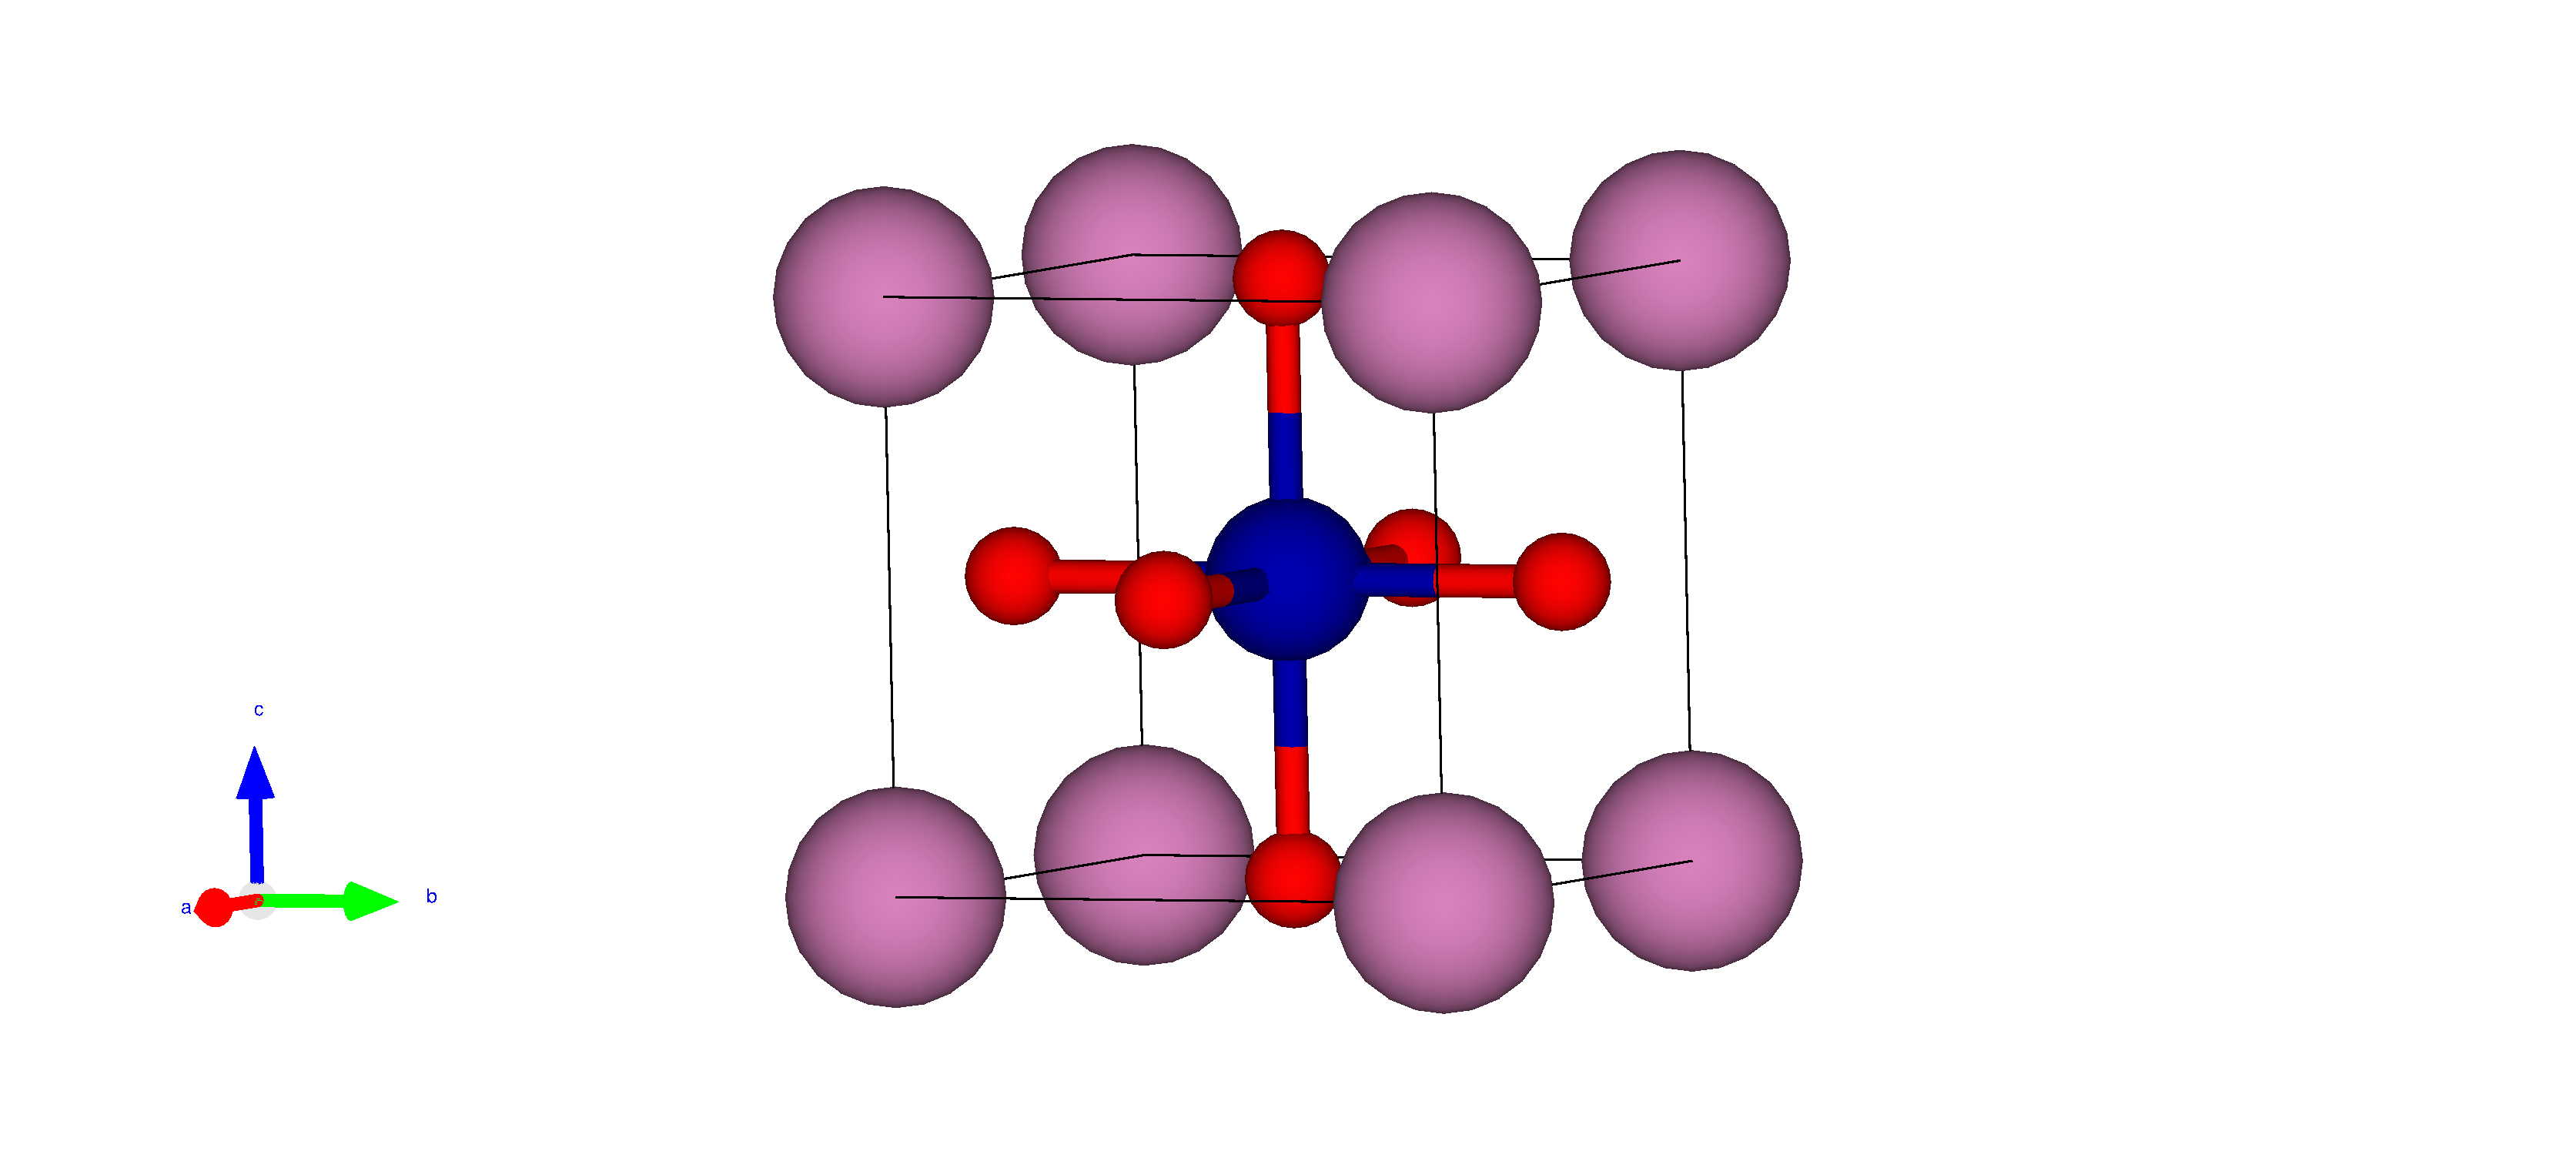
\includegraphics[width=\textwidth]{InCoO3}
    \end{adjustbox}

    \begin{adjustbox}{center,caption={Cubic Structure of InFeO3},label={somelabel},nofloat=figure,vspace=\bigskipamount}
        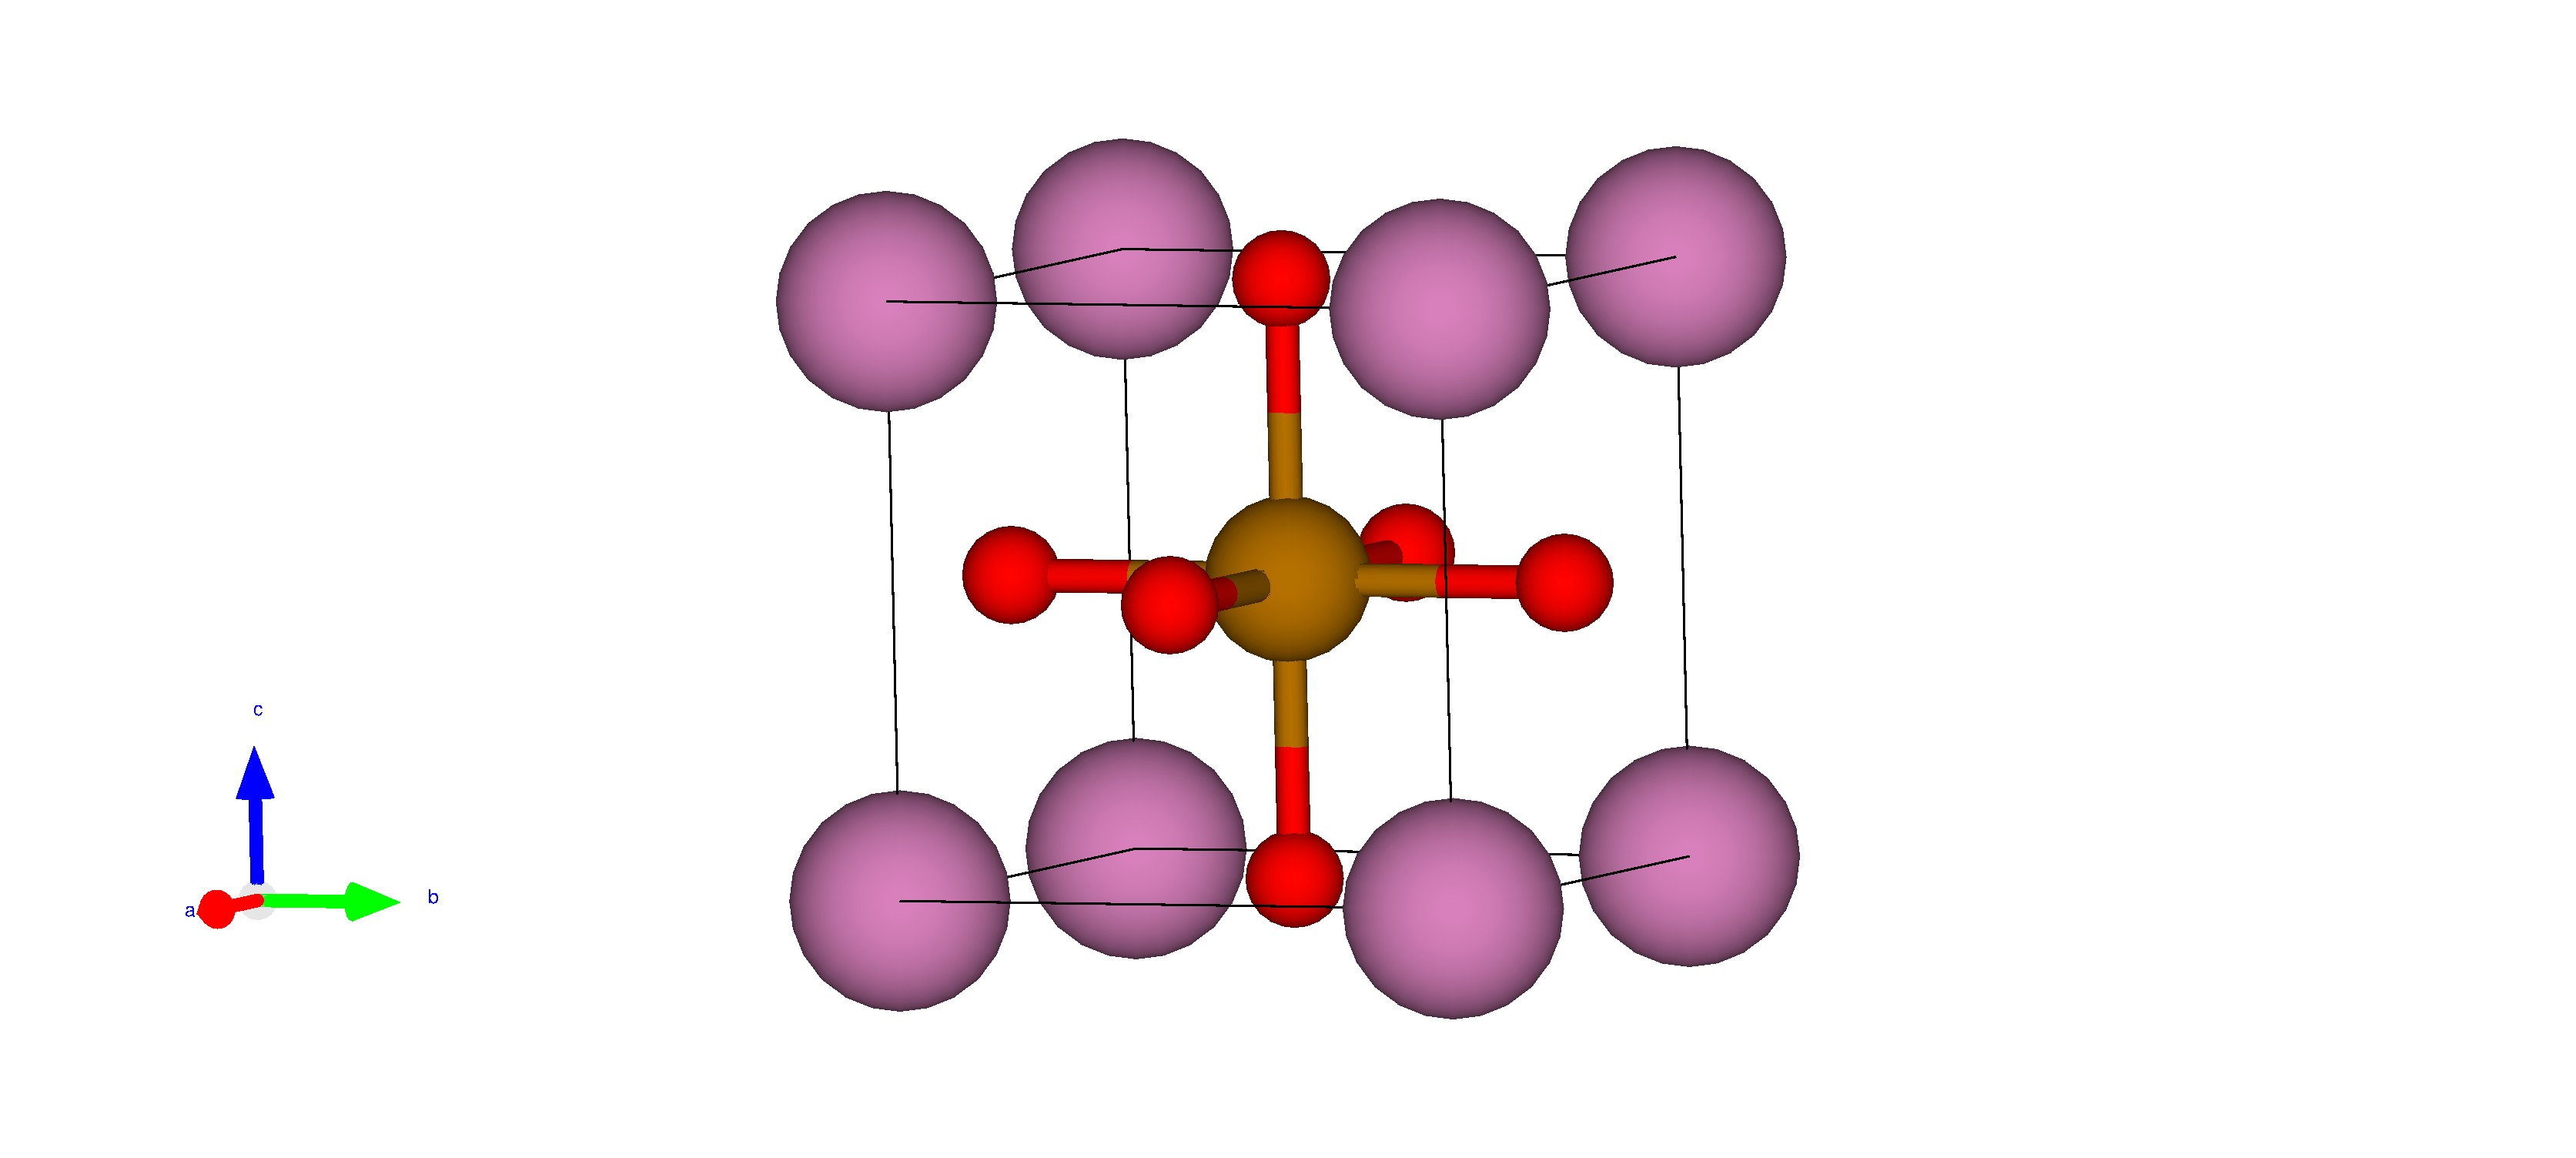
\includegraphics[width=\textwidth]{InFeO3}
    \end{adjustbox}

    \begin{adjustbox}{center,caption={X-Ray diffraction pattern of InCoO3},label={somelabel},nofloat=figure,vspace=\bigskipamount}
        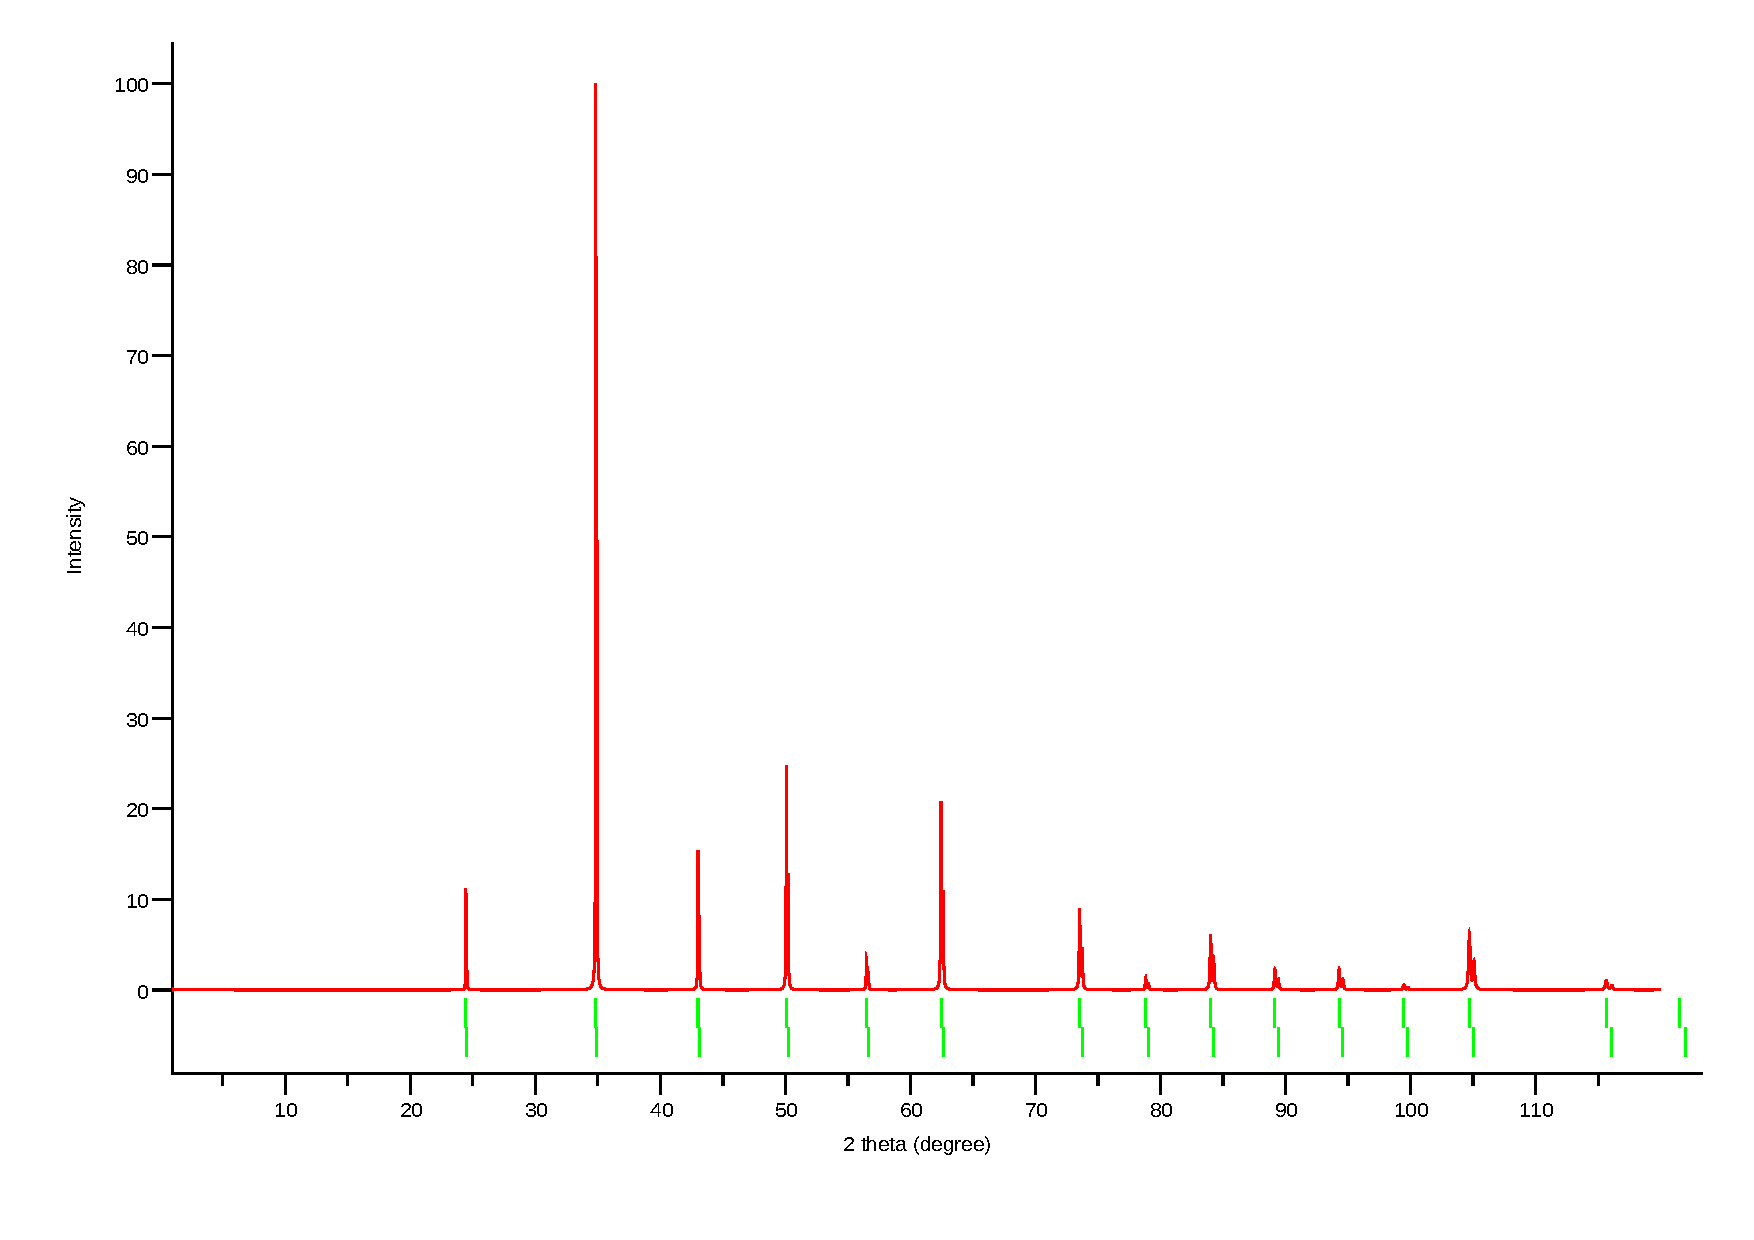
\includegraphics[width=\textwidth]{POSCARCo}
    \end{adjustbox}
    

    \begin{adjustbox}{center,caption={X-Ray diffraction pattern of InFeO3},label={somelabel},nofloat=figure,vspace=\bigskipamount}
        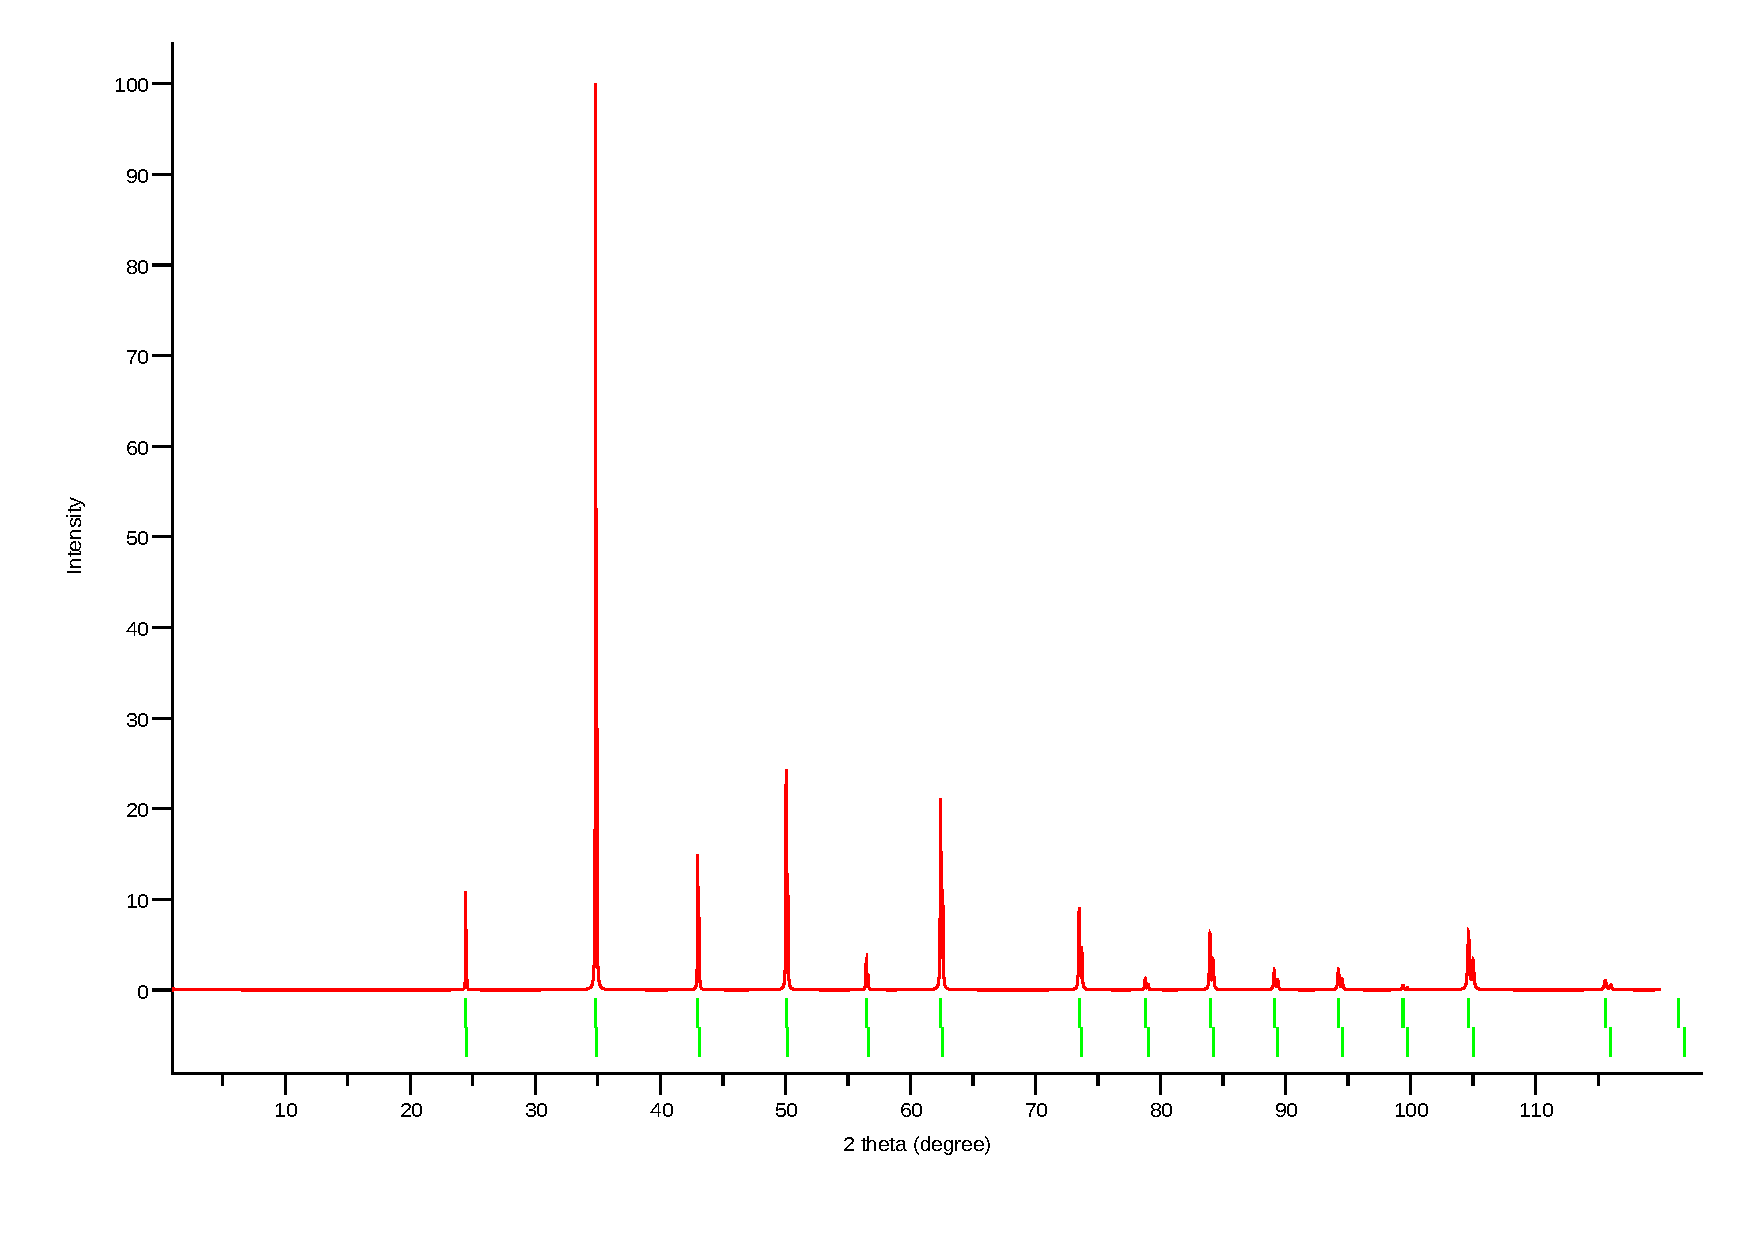
\includegraphics[width=\textwidth]{POSCARFe}
    \end{adjustbox}

    In this type of material, O is oxygen with (-2) ionic valence anion, and A and B metal 
    cations give (+6) valence ion combined. Perovskite material family has numerous types of oxide form like transition metal oxides with the general formula of ABO3\cite{r2}.
    One perovskite material is LiNbO3. For that, we took LiNbO3-like material InCoO3, InFeO3 and sampled magnetic and optical properties with DFT calculations\cite{r3}. 
    
    \section{Computaion Method}
    During the past decade, computer simulations based on a quantum-mechanical description of the interactions between electrons 
    and between electrons and atomic nuclei have developed an increasingly important impact on solid-state physics and chemistry 
    and on materials science—promoting not only a deeper understanding, but also the possibility to contribute significantly to 
    materials design for future technologies. This development is based on two important columns: \\
    
    (i) The improved description of electronic many-body effects within density-functional theory (DFT) and the upcoming post-DFT 
    methods. \\ 
    (ii) The implementation of the new functionals and many-body techniques within highly efficient, stable, and versatile 
    computer codes, which allow to exploit the potential of modern computer architectures. \\ 

    An understanding of mathematical functions and functionals is
    required to understand the basic language of DFT\cite{r15}. Functions
    take a number as input and yield a number as output. For
    example, eq 1, could take x = 2 as input and yield f(x) = 4 as
    output. Functionals are functions of functions. Functionals take
    a function as input and yield a number as output. The input for
    a function is enclosed in parentheses (for example f(x)),
    whereas the input for a functional is enclosed in square brackets
    (for example F[y]). A very simple functional is the definite
    integral functional, F[y] that yields the area under any provided
    function, y. For example, let us say that we are interested in the
    area under any general curve, y = f(x), from x = 0 to x = 3. The
    functional, F[y], is then given by 
    
    \begin{equation}
        y = f(x) = 2x
    \end{equation}
    
    \begin{equation}
        F[y] = \int ^{3} _{0} f(x) dx
    \end{equation}
    
    The functional F[y] in eq 2 could take the function given in
    eq 1 as input and yield the output F[2x] = 9. Functionals can
    be defined as either local or nonlocal. A functional is local if the
    functional’s value can be computed for small segments of the
    input curve and then summed to find the total value. Other-
    wise the functional is called nonlocal. A density functional takes
    the electron density (a function of the position coordinate, r) as
    an input and outputs a number (an energy). Density func-
    tionals can be local or nonlocal. \\ 
     \\ 

    As usual in many-body electronic structure calculations, the nuclei of the treated molecules or clusters are seen as fixed (the Born–Oppenheimer 
    approximation), generating a static external potential V, in which the electrons are moving. A stationary electronic state is then described by a 
    wavefunction $\psi (r1, …, rN)$ satisfying the many-electron time-independent Schrödinger equation. 
    \begin{equation}
        \begin{split}
        \hat{H} \Psi & = \left[\hat{T} + \hat{V} + \hat{U} \right] \\
        & =\left[\sum ^{N} _{i=1}\left(-\frac{\hbar}{2m_{i}}\Delta ^{2}_{i}\right)+ \sum^{N}_{i=1}V(r_{i})+\sum^{N}_{i<j}U(r_{i},r_{j})\right]\Psi = E\Psi
        \end{split}
    \end{equation}

    where, for the N-electron system, $\hat{H}$ is the Hamiltonian, E is the total energy, $\hat{T}$ is the kinetic energy, $\hat{V}$
    is the potential energy from the external field due to positively charged nuclei, and $\hat{U}$ is the electron-
    electron interaction energy. As $\hat{T} \hat{U}$ is equal for any N-electron system, they are called universal operator.
    Only $\hat{V}$ is system-dependent. This complicated many-particle equation is not detachable
    into simpler single-particle equations beacuse of the interaction term $\hat{U}$.
    There are numerous cultivated processes for translating the many-body 
    Schrödinger equation based on the development of the wavefunction in Slater determinants While the easiest one is the Hartree–Fock method, more cultivated techniques are usually tagged as post-Hartree–Fock
    methods. Nevertheless, the problem with these scenarios is the huge 
    computational effort, which renders it practically incomprehensible to apply them 
    efficiently to more considerable, more complex techniques.
    separable. Here DFT supplies an adorable alternative, being vastly more universal, 
    as it supplies a way to systematically map the many-body issue, with $\hat{U}$, onto a single-
    body problem without $\hat{U}$, onto a single-body problem without $\hat{U}$. In DFT the key variable
    is the electron density n(r), which for a normalized $\Psi$ is given by 

    \begin{equation}
        n(r) = N \int d^{3}r_{2} ..... \int d^{3}r_{N}\Psi^{*}(r_{1},r_{2},....,r_{n})\Psi(r_{1},r_{2},....,r_{n})
    \end{equation}

    In this review, I discuss the implementation of various DFT functionals [local-density approximation (LDA), generalized gradient approximation (GGA), 
    meta-GGA, hybrid functional mixing DFT, and exact (Hartree-Fock) exchange] and post-DFT approaches 
    [DFT + U for strong electronic correlations in narrow bands, many-body perturbation theory (GW) for quasiparticle spectra, 
    dynamical correlation effects via the adiabatic-connection fluctuation-dissipation theorem (AC-FDT)] in the 
    Vienna ab initio simulation package VASP. \\ 

    For computing the magnetic and optical properties of InFeO3 and InCoO3, we execute Density Functional Theory (DFT)\cite{r5,r6,r7,r8} simulations by  Vienna ab initio Simulation 
    Package (VASP)\cite{r9,r10,r11}. The unit cells of InCoO3 and InFeO3 in the cubic form are shown in Fig. 1, which we explored further. First, we perform structural relaxation. 
    Then we execute static calculation for density of states, band, and optical properties of chosen materials. 
    
%    \begin{figure}[h]
%
%        \begin{subfigure}{0.5\textwidth}
%        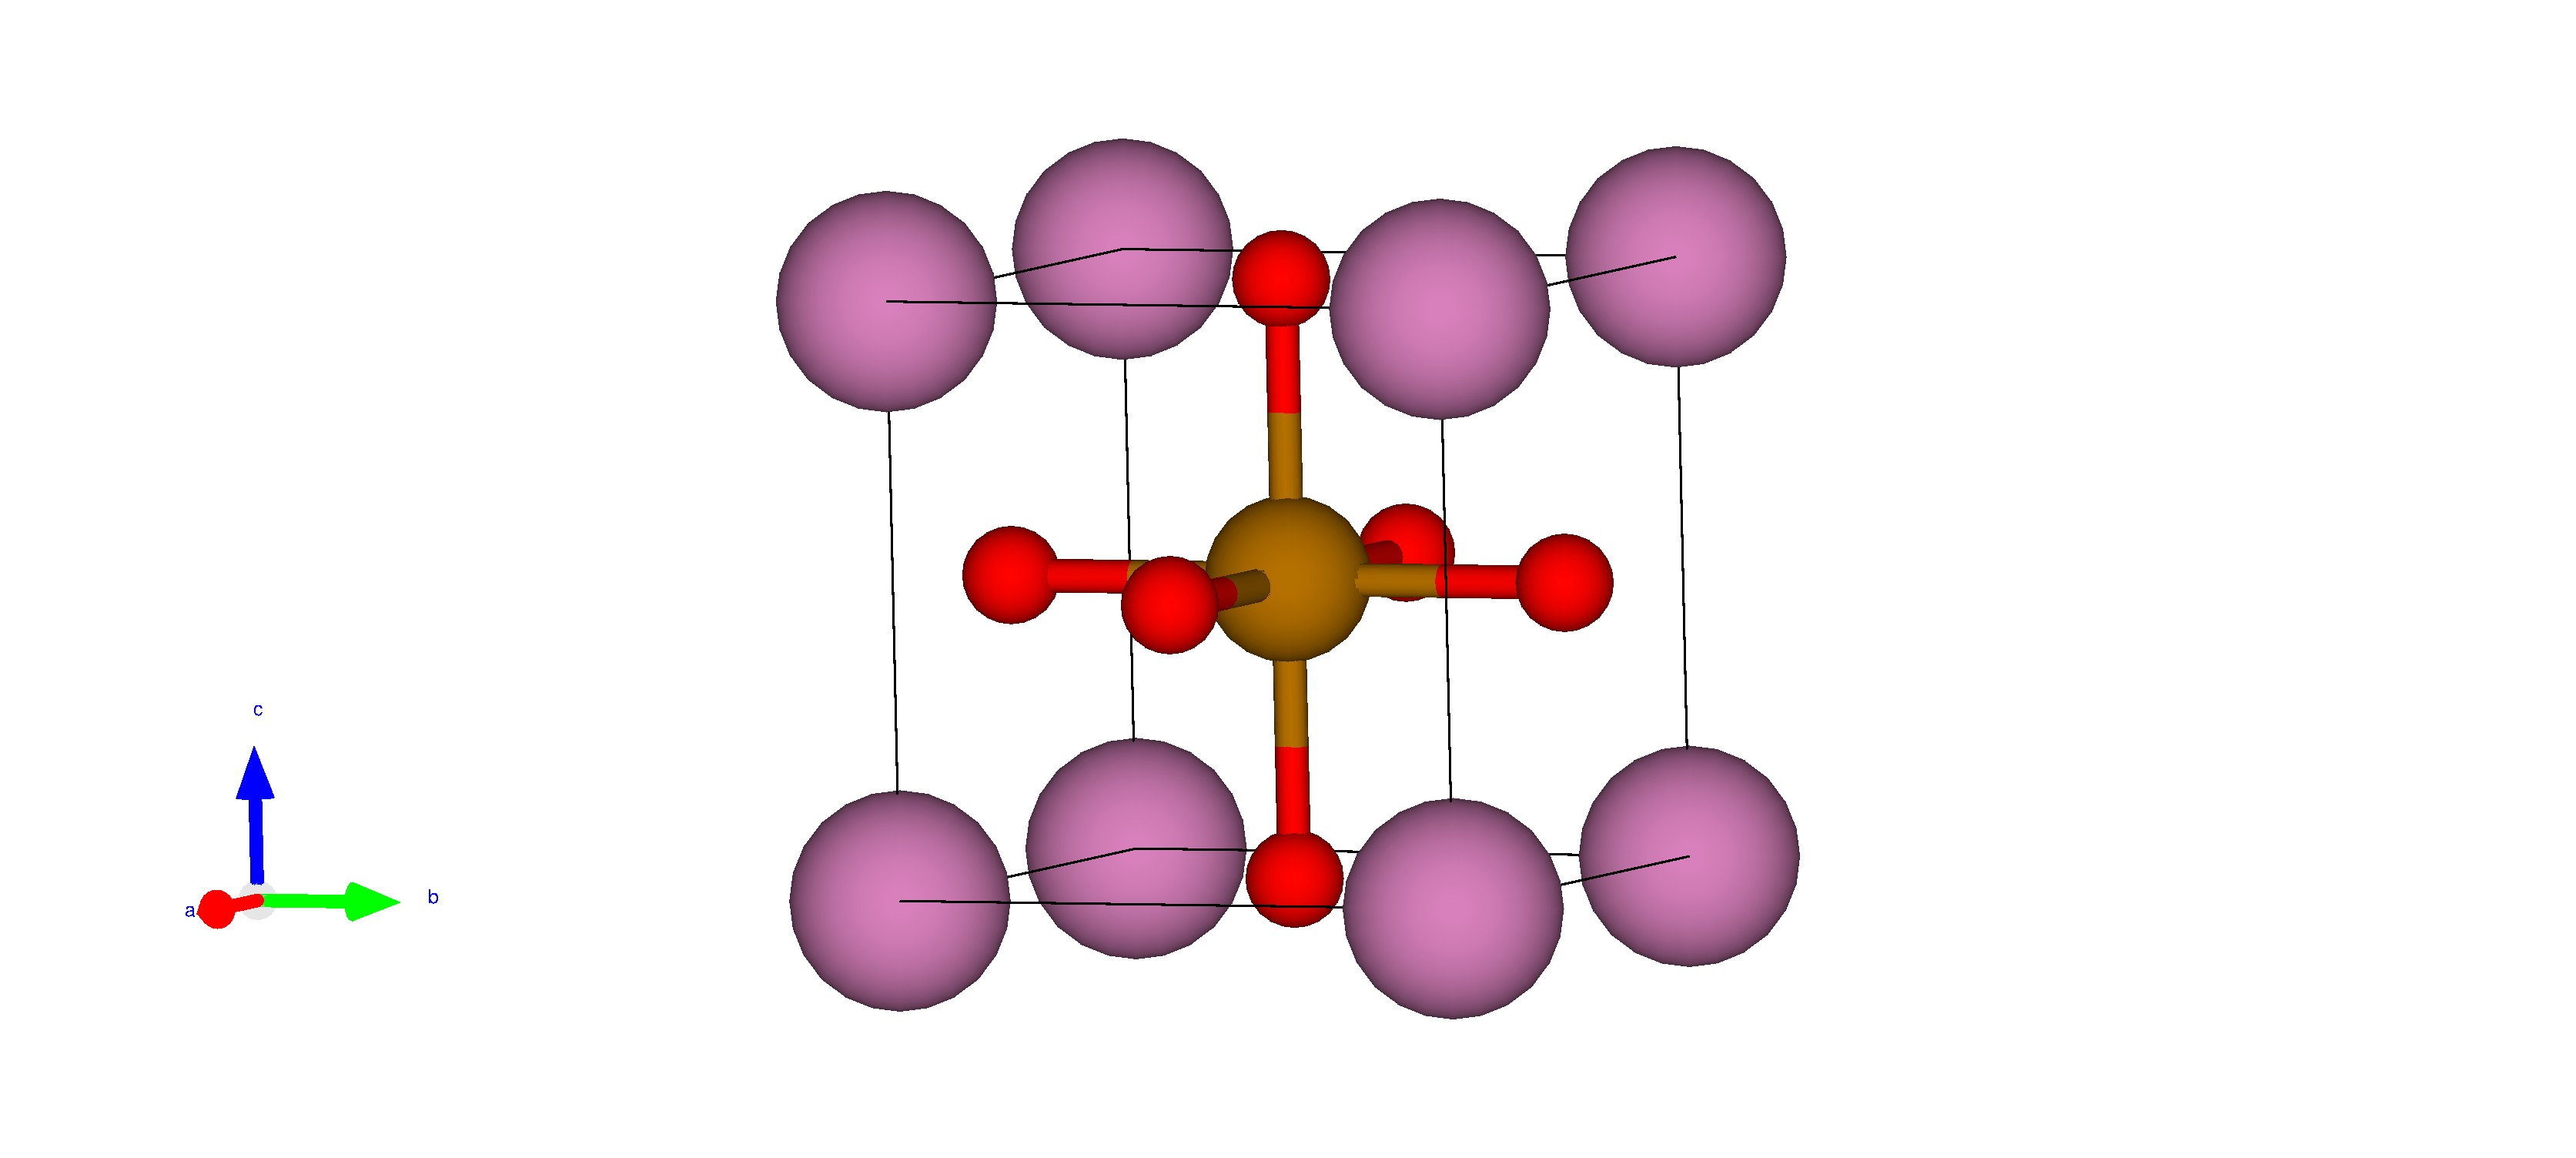
\includegraphics[width=0.4\paperwidth, height=6cm]{InFeO3}
%        \caption{Caption1}
%        \label{fig:subim1}
 %       \end{subfigure}
 %       \begin{subfigure}{0.5\textwidth}
 %       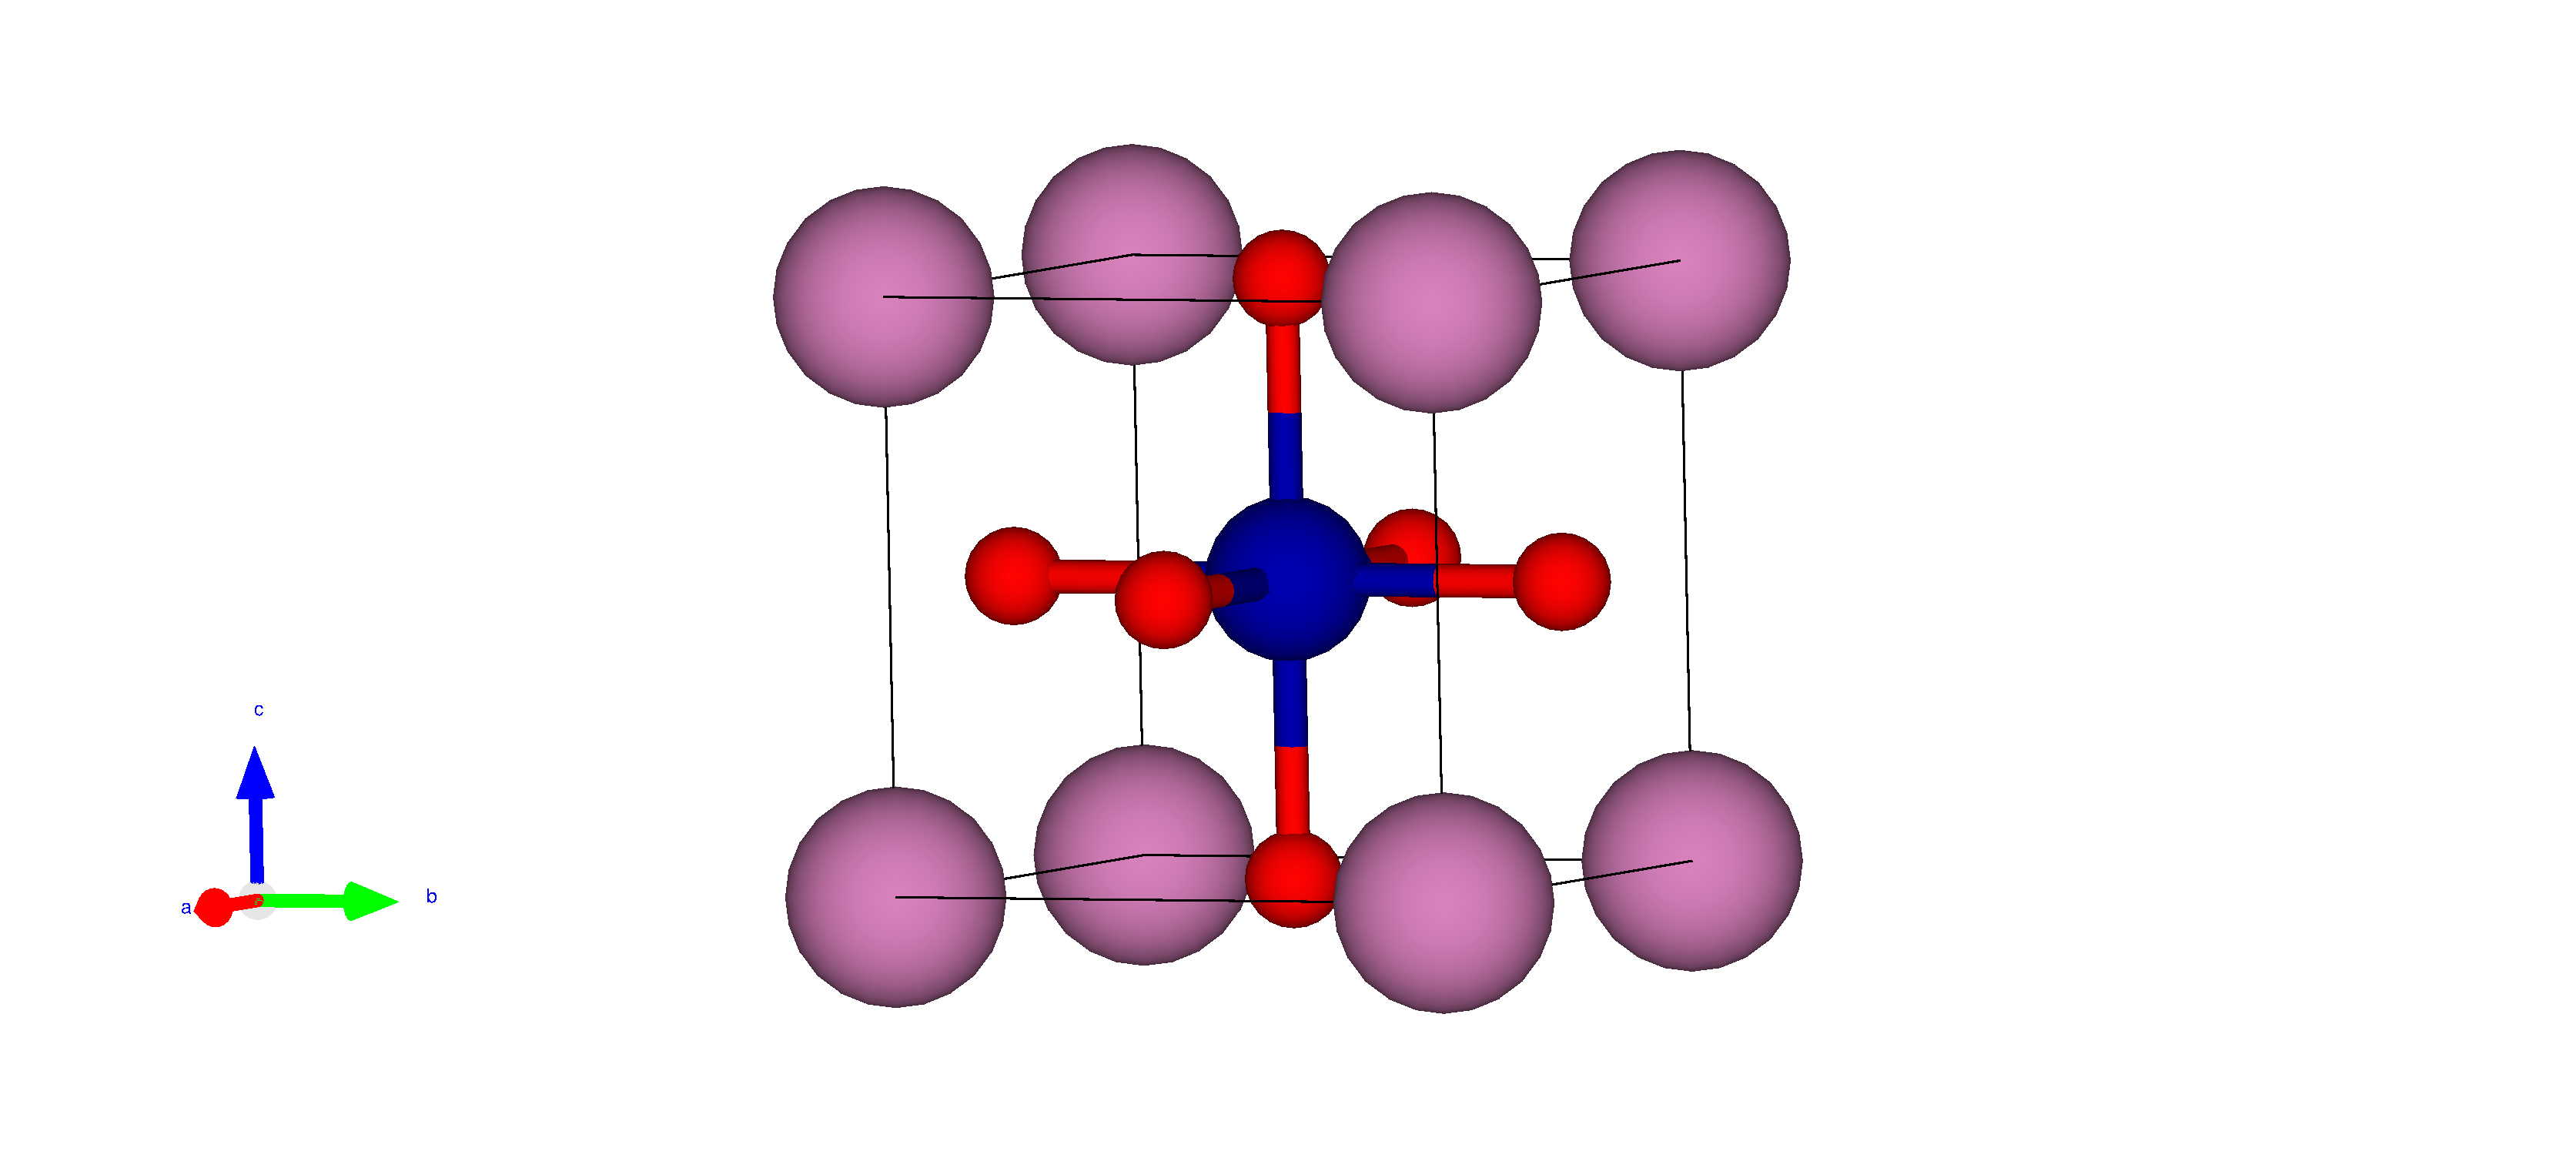
\includegraphics[width=0.4\paperwidth, height=6cm]{InCoO3}
 %       \end{subfigure}
            
    %\end{figure} 
    %\begin{figure}[H]
    %\centering
    %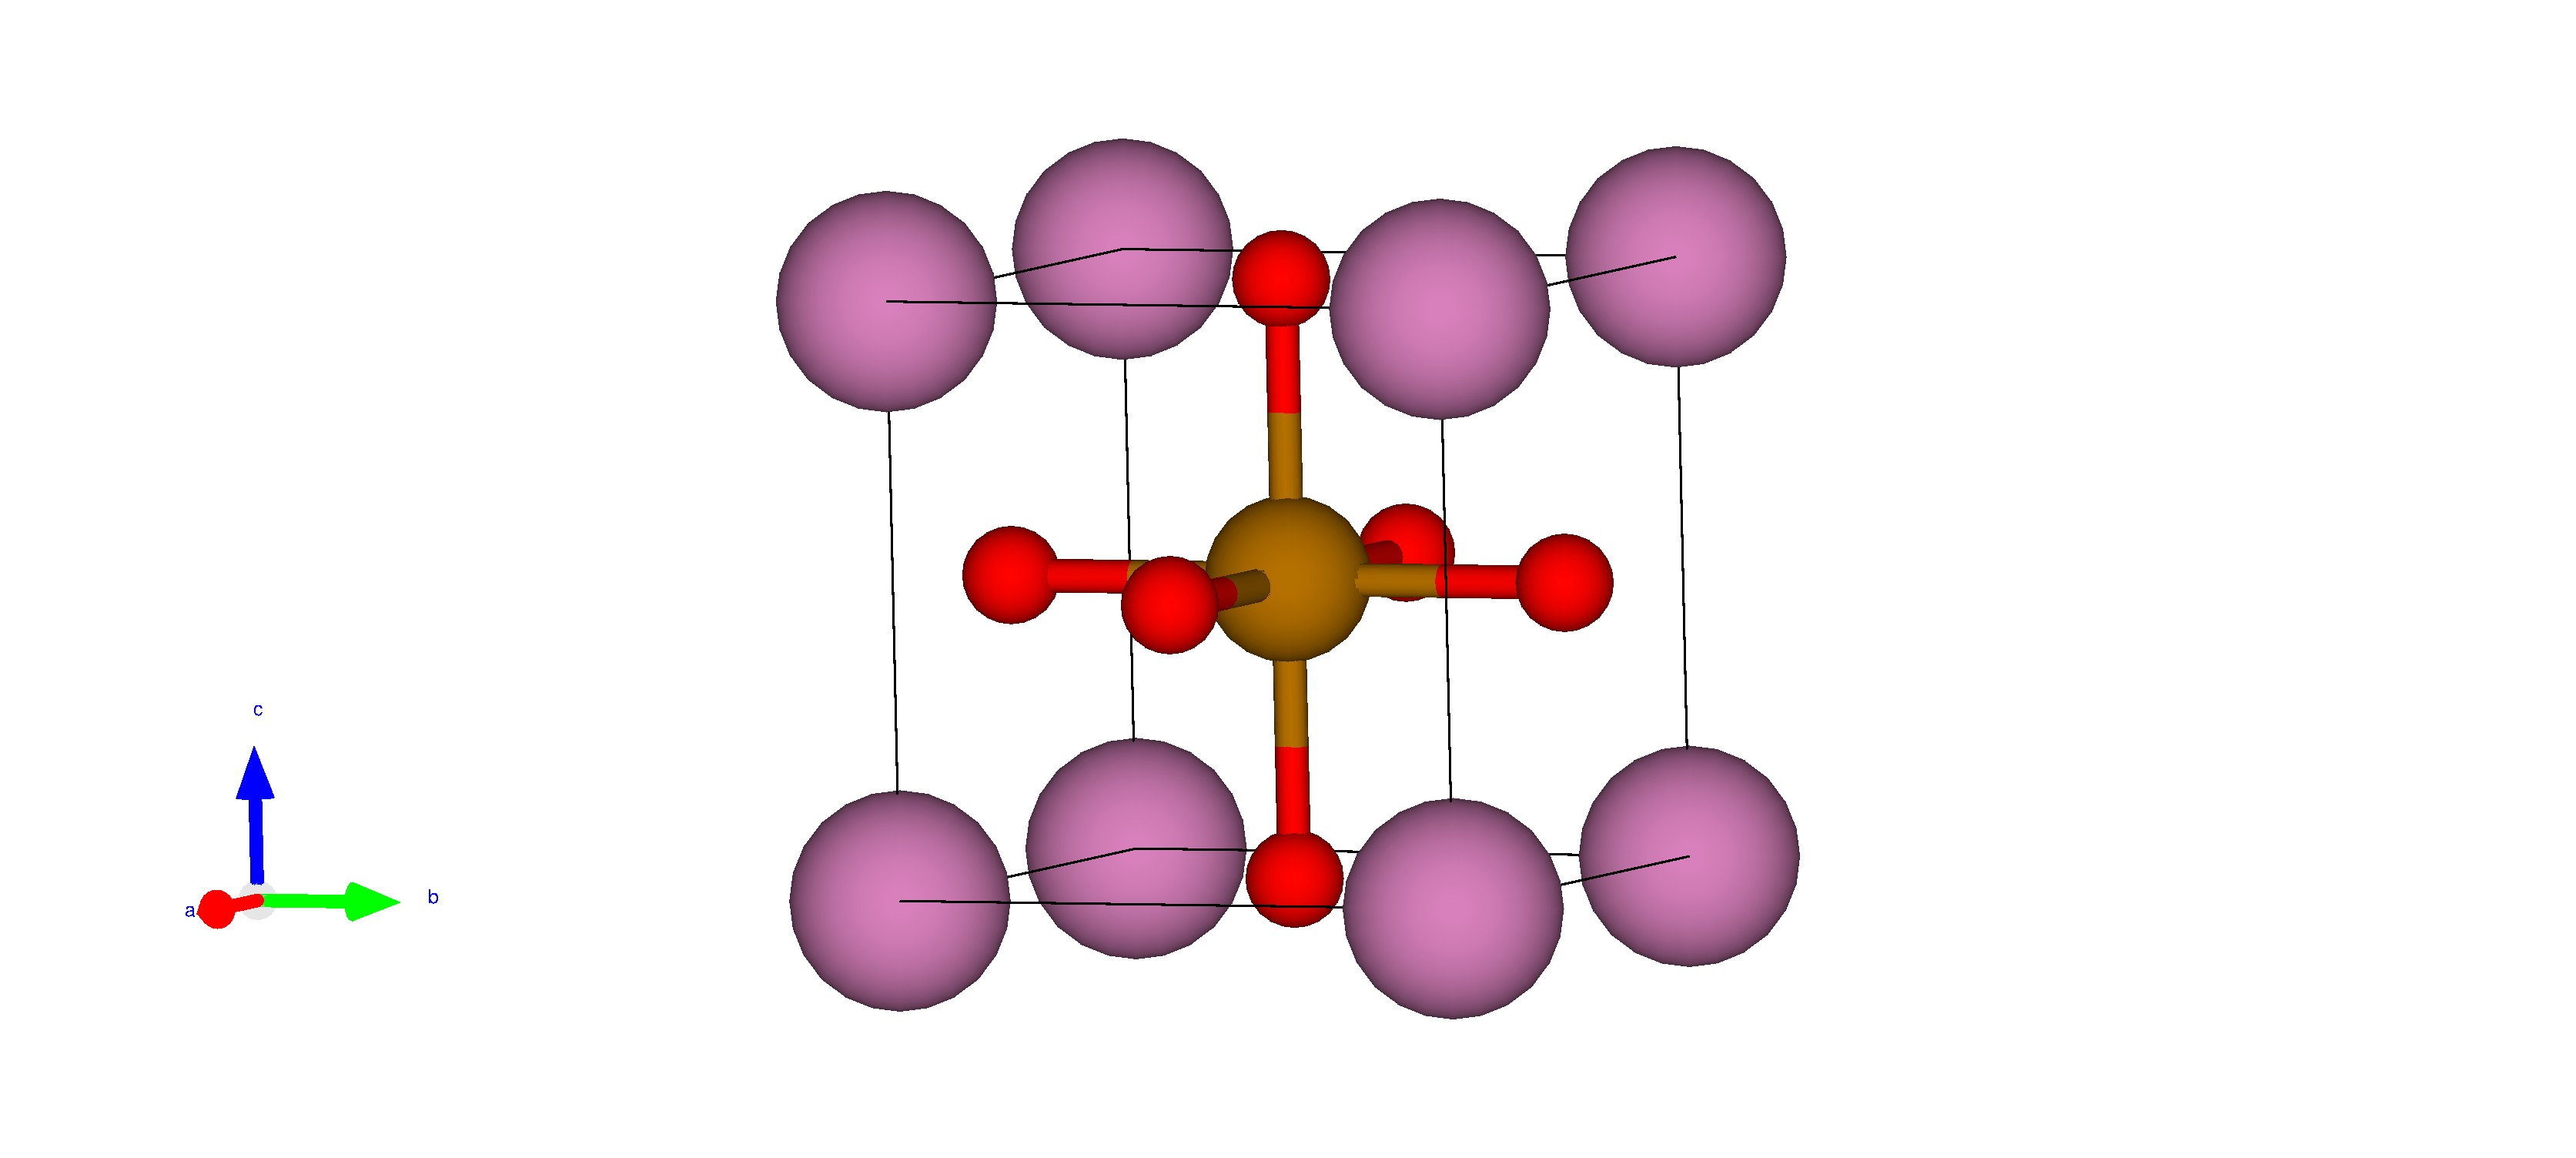
\includegraphics[scale=.3]{InFeO3}
    %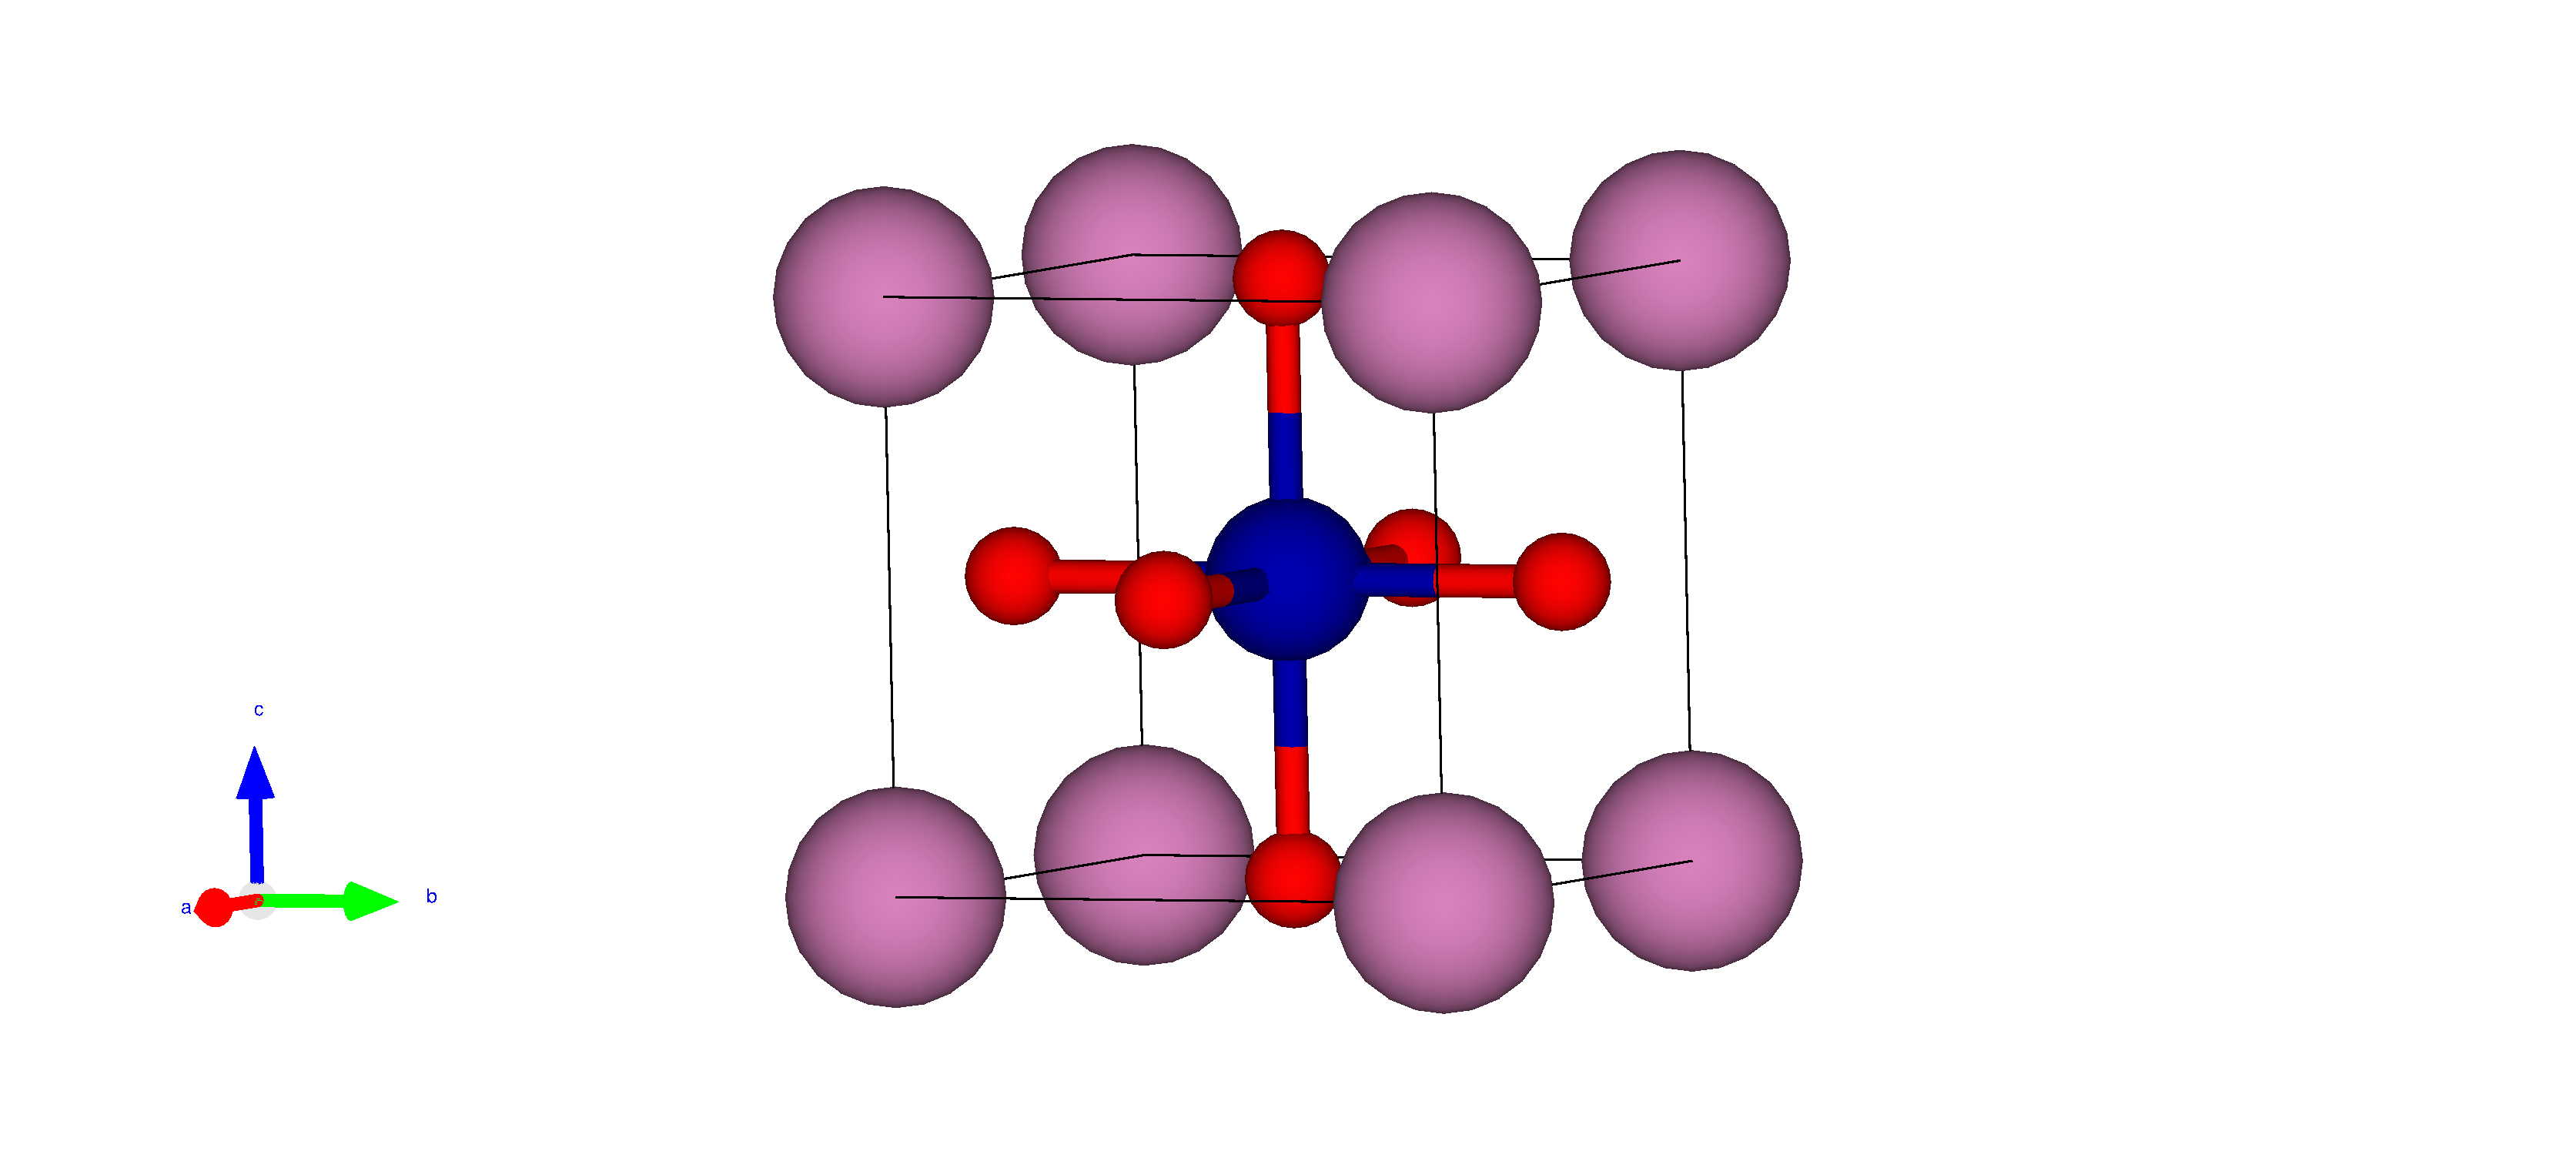
\includegraphics[scale=.3]{InCoO3}
    %\end{figure}

    \begin{adjustbox}{center,caption={Band Structure Of InCoO3},label={somelabel},nofloat=figure,vspace=\bigskipamount}
        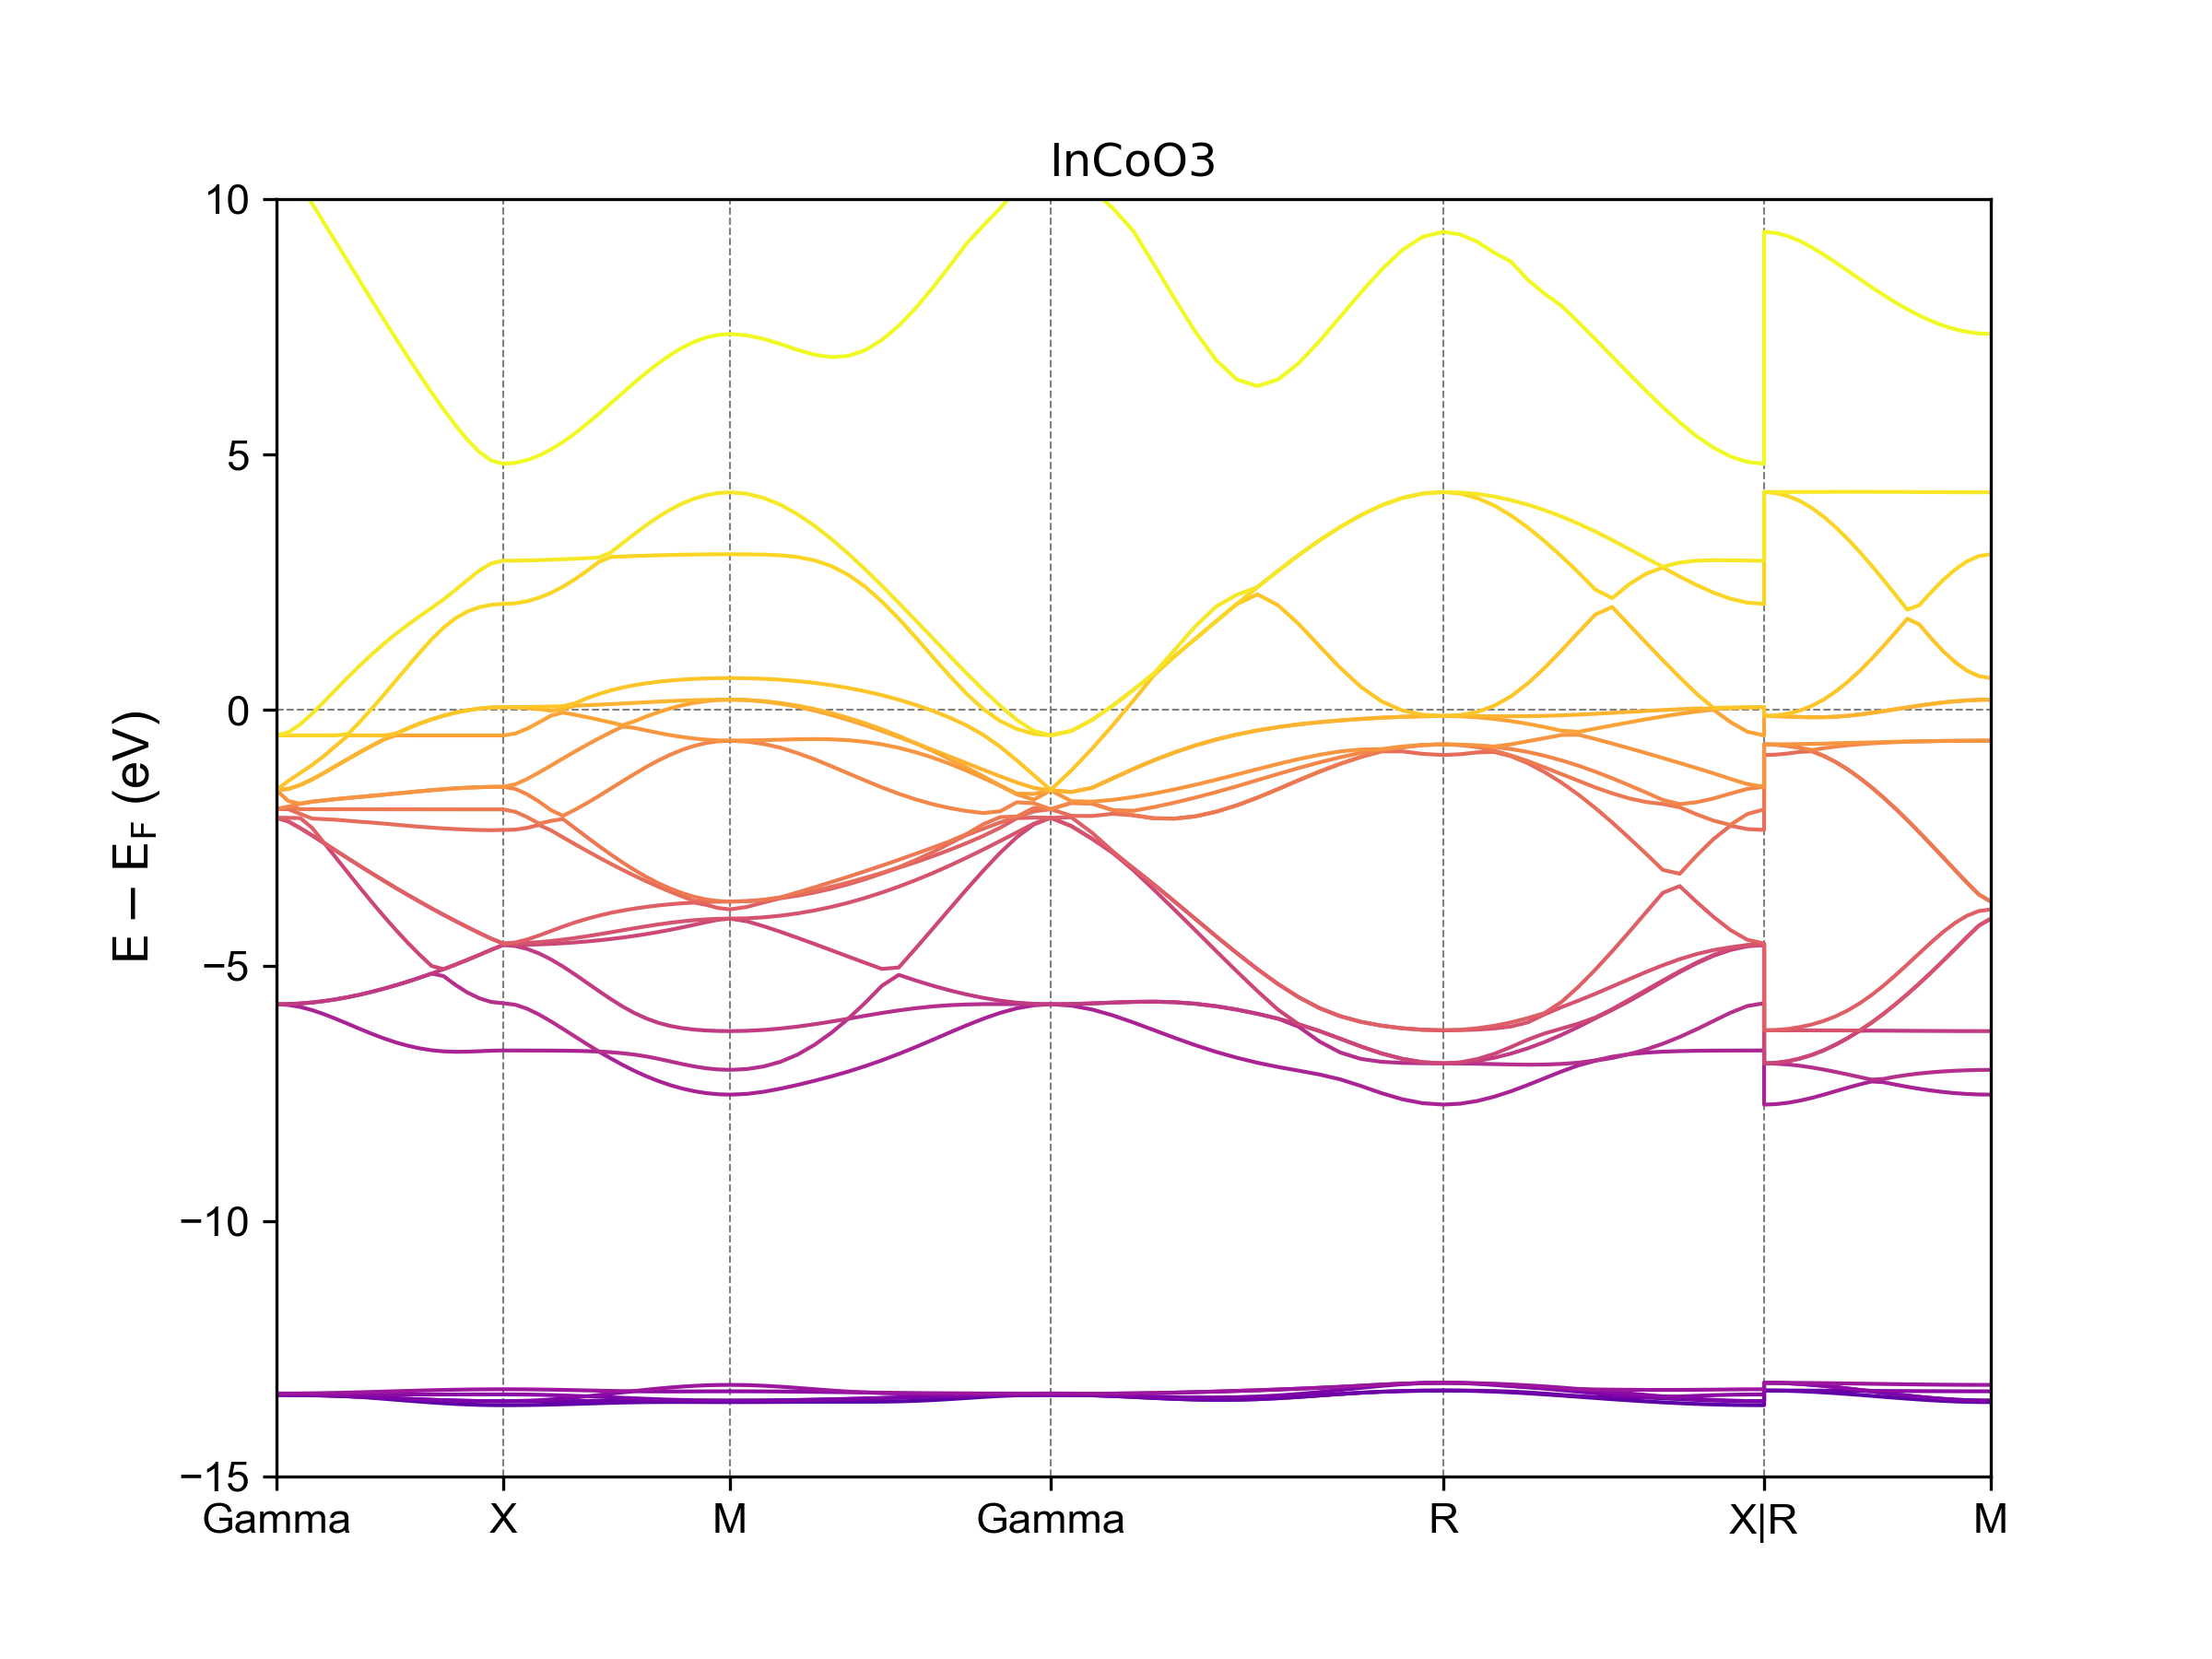
\includegraphics[width=\textwidth]{bandCo}
    \end{adjustbox}

    \begin{adjustbox}{center,caption={Band Structure Of InFeO3},label={somelabel},nofloat=figure,vspace=\bigskipamount}
        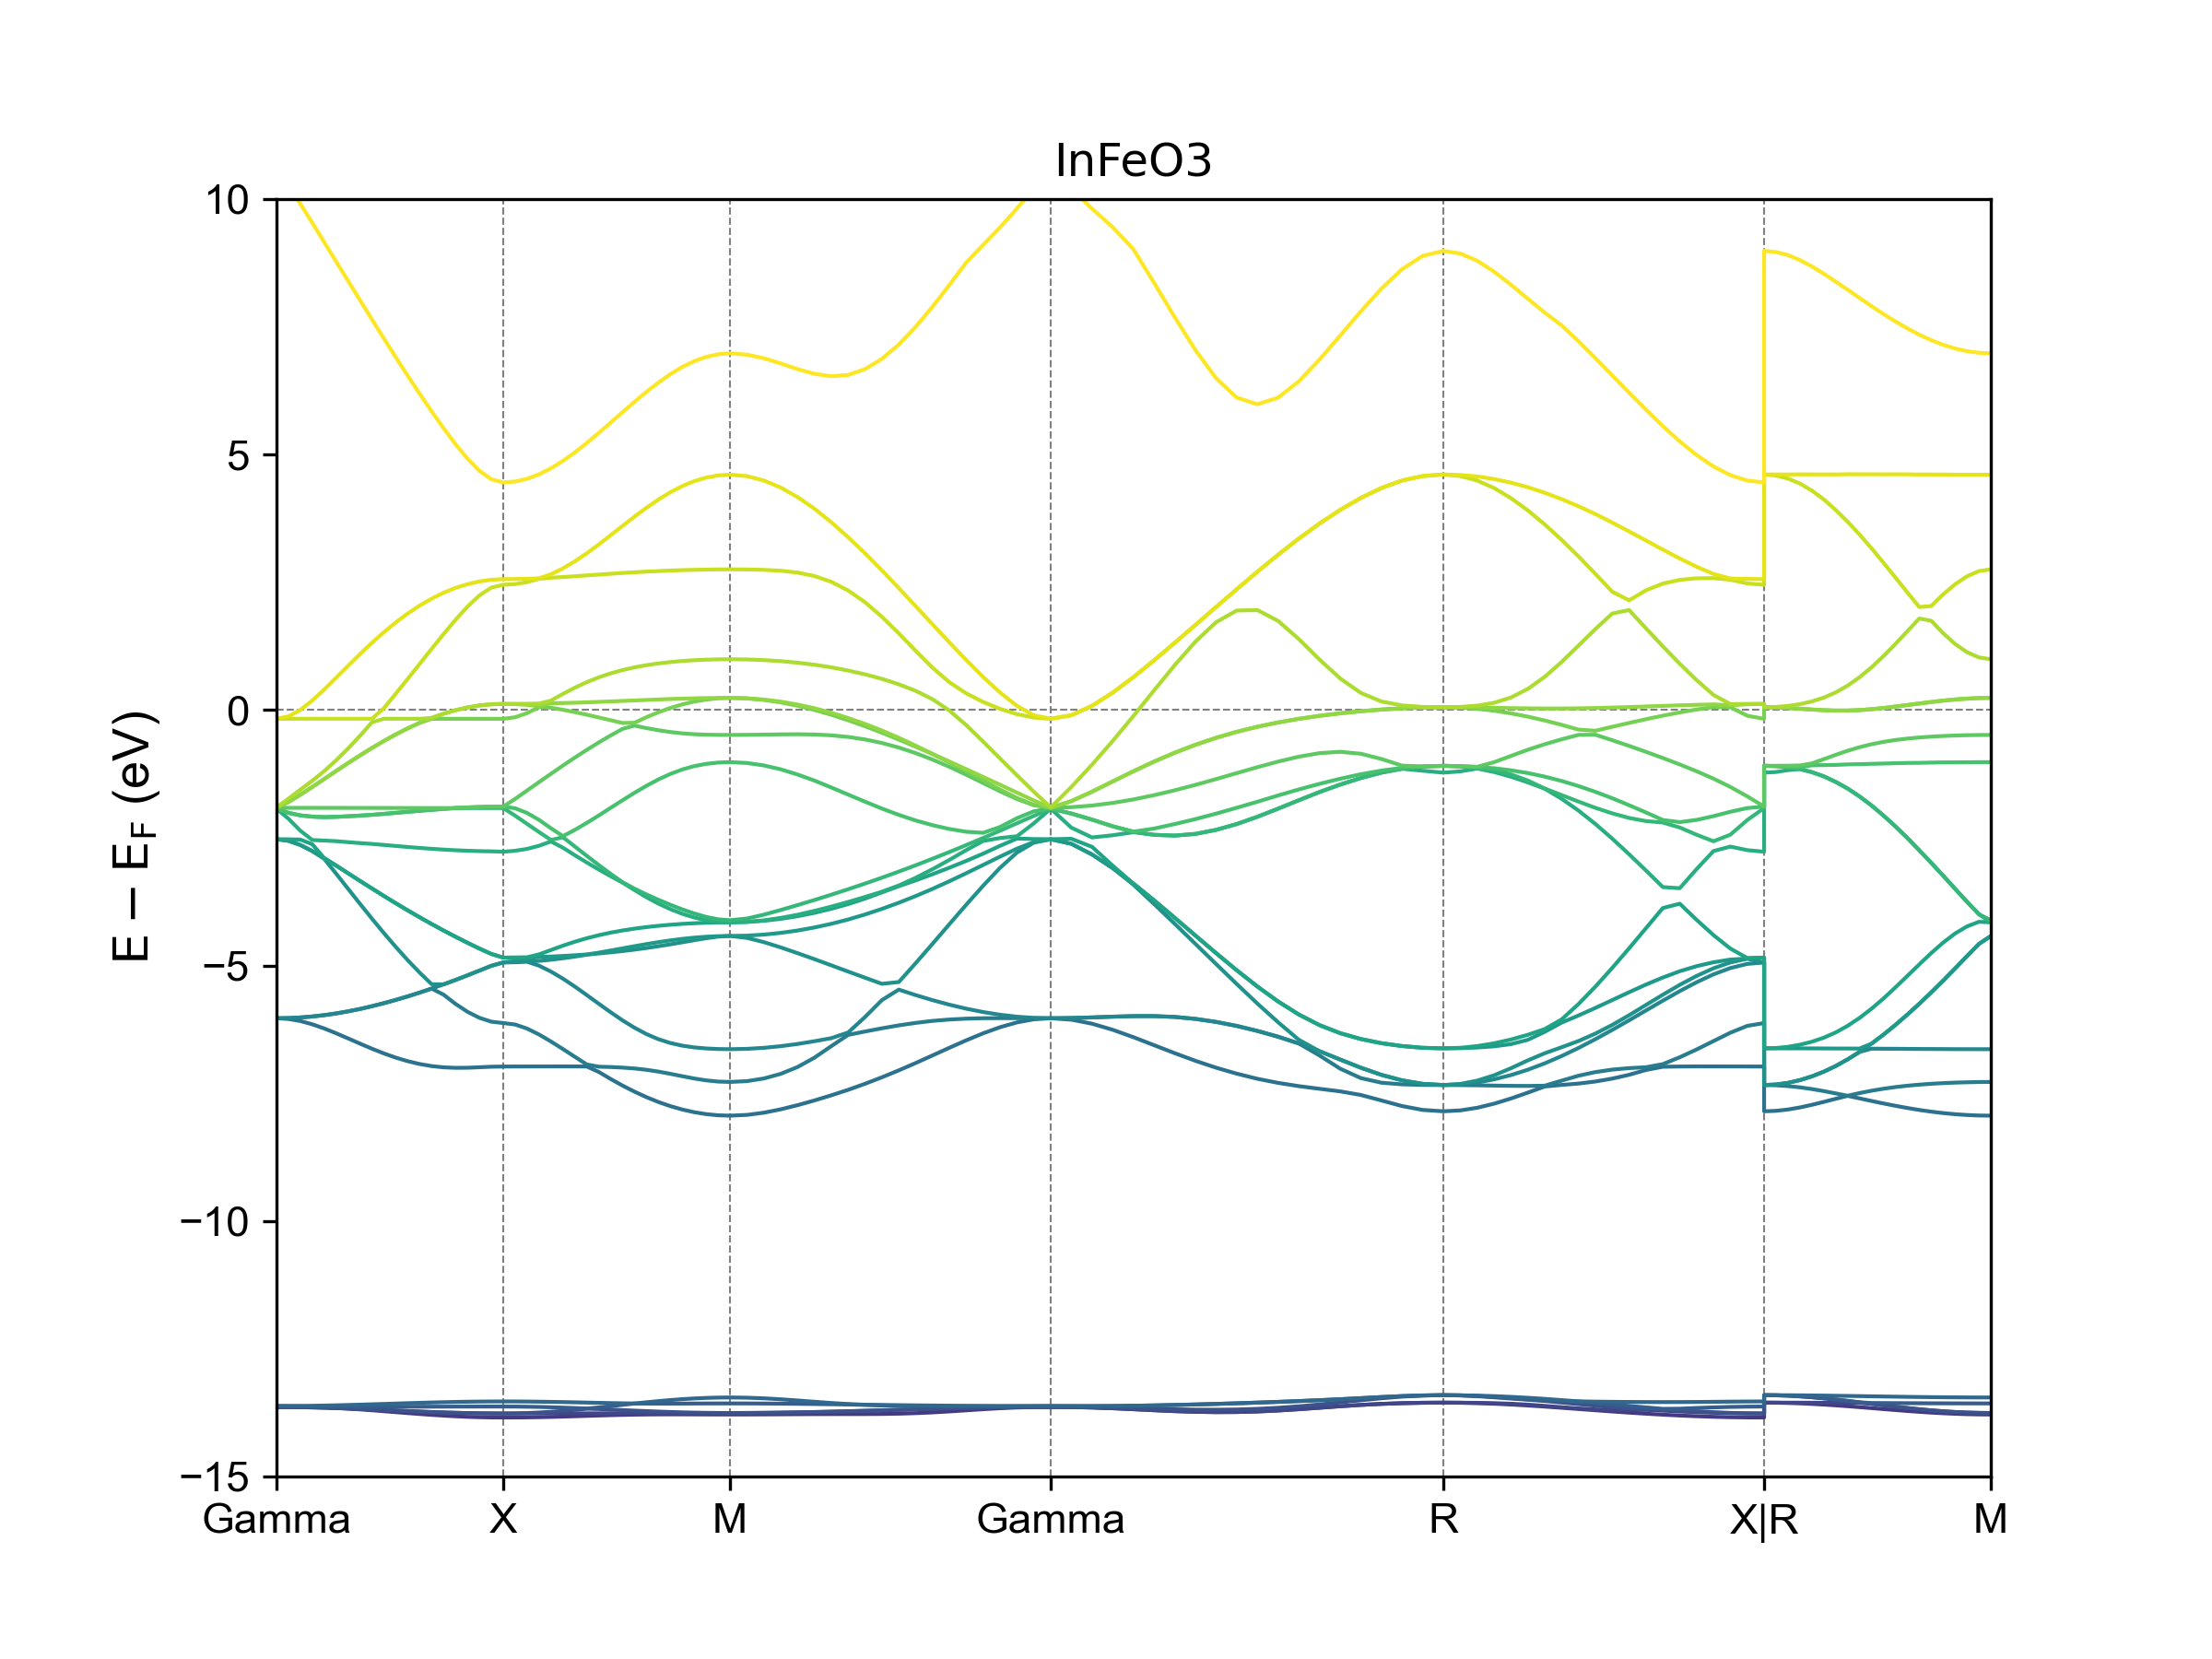
\includegraphics[width=\textwidth]{bandFe}
    \end{adjustbox}

    \section{Results}
    InFeO3 and InCoO3 are cubic structures under the space group of Pm3m (no. 221). We visualize the structures in VESTA (3D Visualization for Electronic and 
    Structural Analysis). The unit cell of InCoO3 and InFeO3 constitutes five atoms (shown in Fig. 1). Fe or Co atoms hold the corner positions of the cubes (Wyckoff 
    site (0,0,0)), In situated in the crystal's body-centered positions (Wyckoff site(0.5,0.5,0.5)). O occupies face-centered positions (Wyckoff site (0.5,0.5,0)). 
    The electronic band structures and density of states(DOS) of relaxed InCoO3 and InFeO3 structures through PBE functional considering the GGA approximation. 
    Band structures of InCoO3 and InFeO3 are shown in Fig. 2.  


    
    Zero-point energy is Fermi energy.Two structures show indirect bandgap and the range of the bandgap 
    energy resembles that both the structures are metallic in nature. The outcome of the bandgaps and band structures of the examined materials confirm their wonder
    for photothermal, photovoltaic, and optoelectronic applications. InCoO3 and InFeO3 show the same bandgap. The density of states of atoms is shown in Fig. 3.
    
    \begin{adjustbox}{center,caption={Density of States Of InCoO3},label={somelabel},nofloat=figure,vspace=\bigskipamount,}
        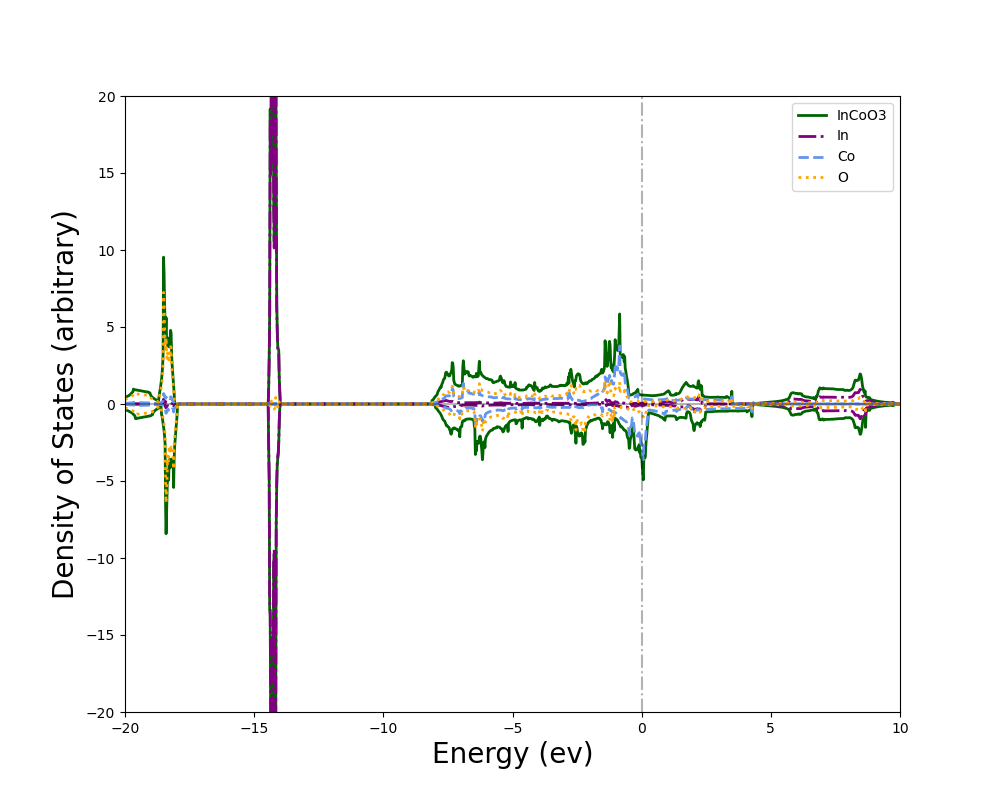
\includegraphics[width=\textwidth]{DosInCoO3}
    \end{adjustbox}

    \begin{adjustbox}{center,caption={Density of States Of InFeO3},label={somelabel},nofloat=figure,vspace=\bigskipamount,}
        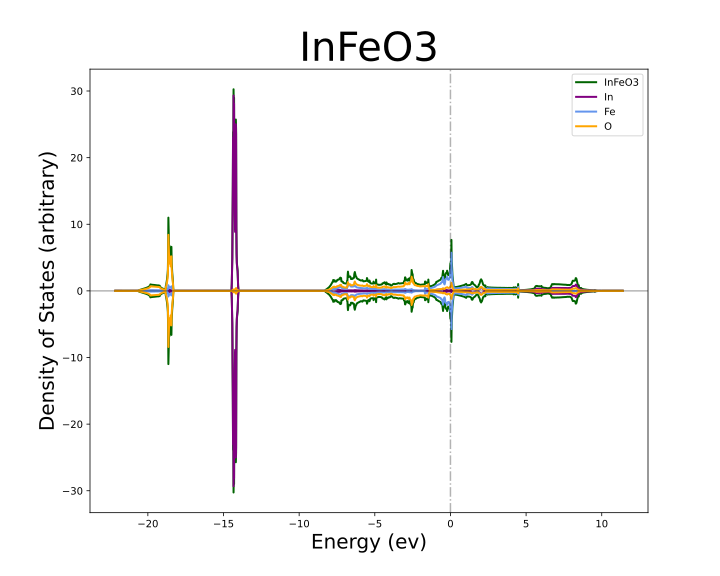
\includegraphics[width=\textwidth]{DosInFeO3}
    \end{adjustbox}
    
    The orbital projected density of states indicates at the Fermi level, the p-orbital of Co and Fe atom is the main benefactor. The optical properties of a 
    material rely on many parts. Such as absorption spectra, concerning light energy and wavelength, reflectivity, refractivity index, dielectric constants, and 
    optical conductivity. We examined these properties with InCoO3 and InFeO3.  The optical absorption coefficient indicates how much light penetrates the substance 
    before being absorbed by the material. This is a piece of important knowledge for solar-energy conversion efficiency for practical application. In Fig. 4 energy 
    and wavelength-dependent absorption profiles are demonstrated.
    
    \begin{adjustbox}{center,caption={Absorption Of InCoO3 and InFeO3},label={somelabel},nofloat=figure,vspace=\bigskipamount,}
        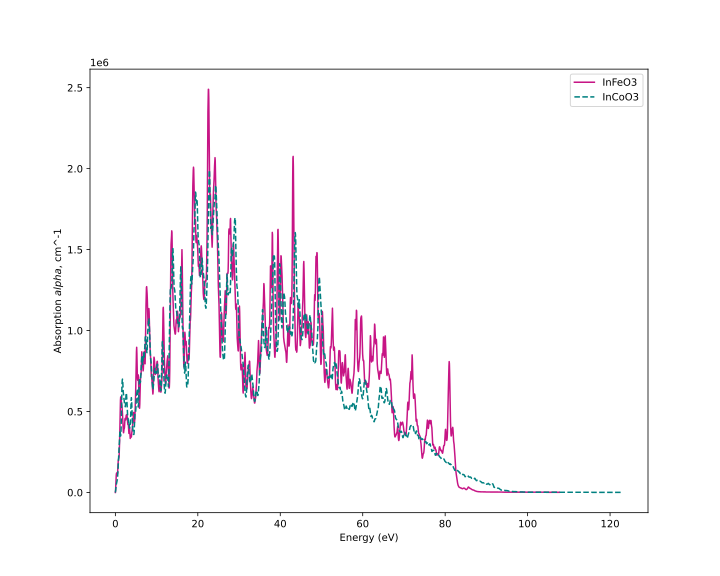
\includegraphics[width=\textwidth]{Absorptioneng}
    \end{adjustbox}
    
    Reflectivity is an optical property to understand the surface nature of the material. It defines 
    how much energy reflects from incident energy on the surface. Fig 5 represents the optical reflectivity of InCoO3 and InFeO3. 
    
    \begin{adjustbox}{center,caption={Reflectivity Of InCoO3 and InFeO3},label={somelabel},nofloat=figure,vspace=\bigskipamount,}
        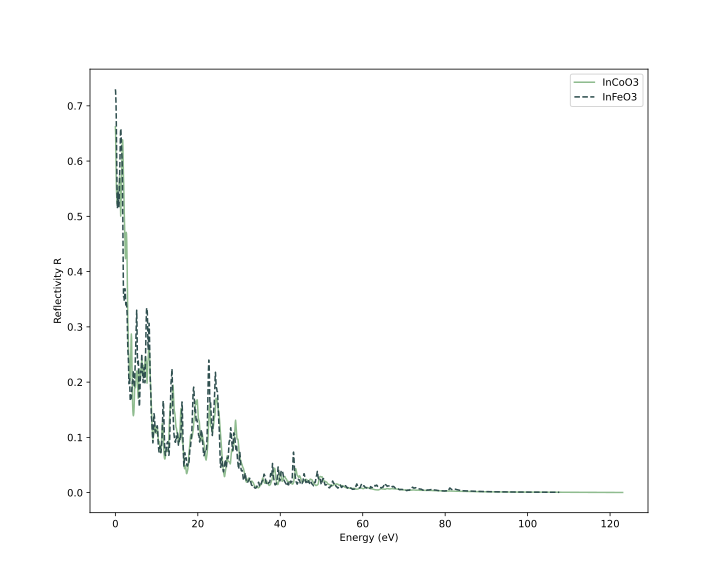
\includegraphics[width=\textwidth]{refleceng}
    \end{adjustbox}
    
    The dielectric constant values are used for determining how well optoelectronic devices work, defined as the response of a material to incident light energy. Higher dielectric values at a lower 
    charge carrier recombination rate are deep in improving the optoelectronic device performance. 

    \begin{adjustbox}{center, caption={Dielectric constants of InCoO3 and InFeO3(Real)},label={somelabel},nofloat=figure,}
        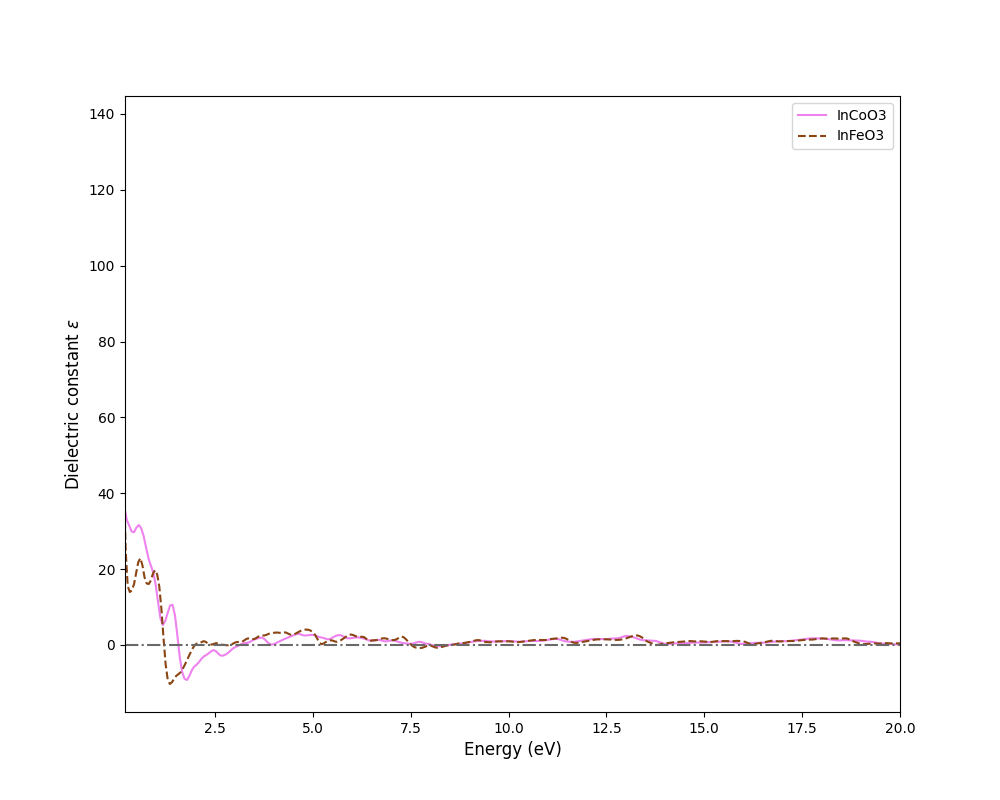
\includegraphics[width=\textwidth]{dieleceng}
    \end{adjustbox}

    \begin{adjustbox}{center, caption={Dielectric constants of InCoO3 and InFeO3(Imaginary)},label={somelabel},nofloat=figure,}
        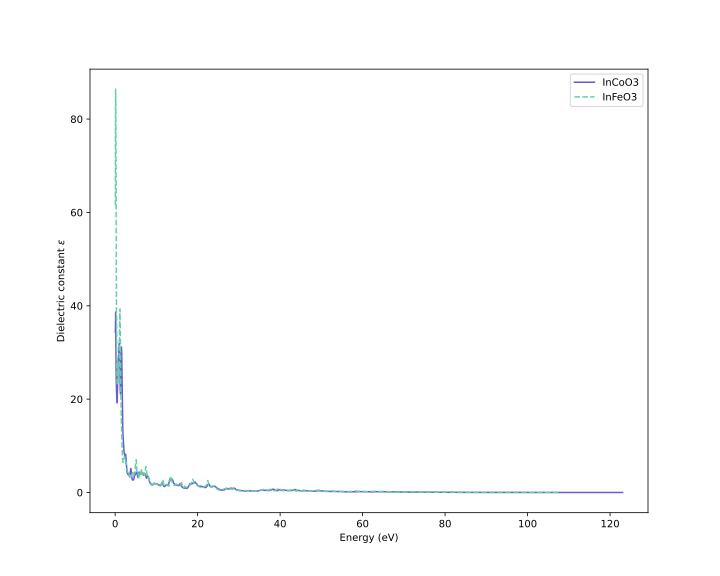
\includegraphics[width=\textwidth]{dielecimageng}
    \end{adjustbox}

    \begin{adjustbox}{center,caption={Optical Conductivity of InCoO3 and InFeO3(Real)},label={somelabel},nofloat=figure,vspace=\bigskipamount}
        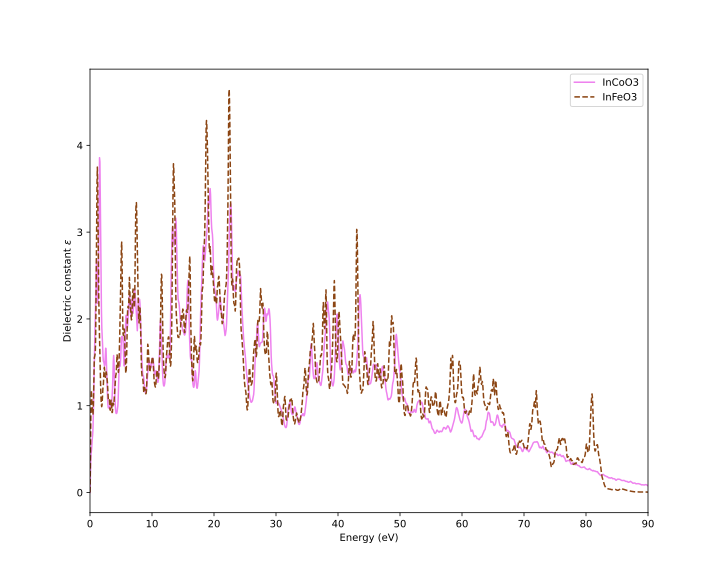
\includegraphics[width=\textwidth]{opcondrealev}
    \end{adjustbox}

    \begin{adjustbox}{center,caption={Optical Conductivity of InCoO3 and InFeO3(Imaginary)},label={somelabel},nofloat=figure,vspace=\bigskipamount}
        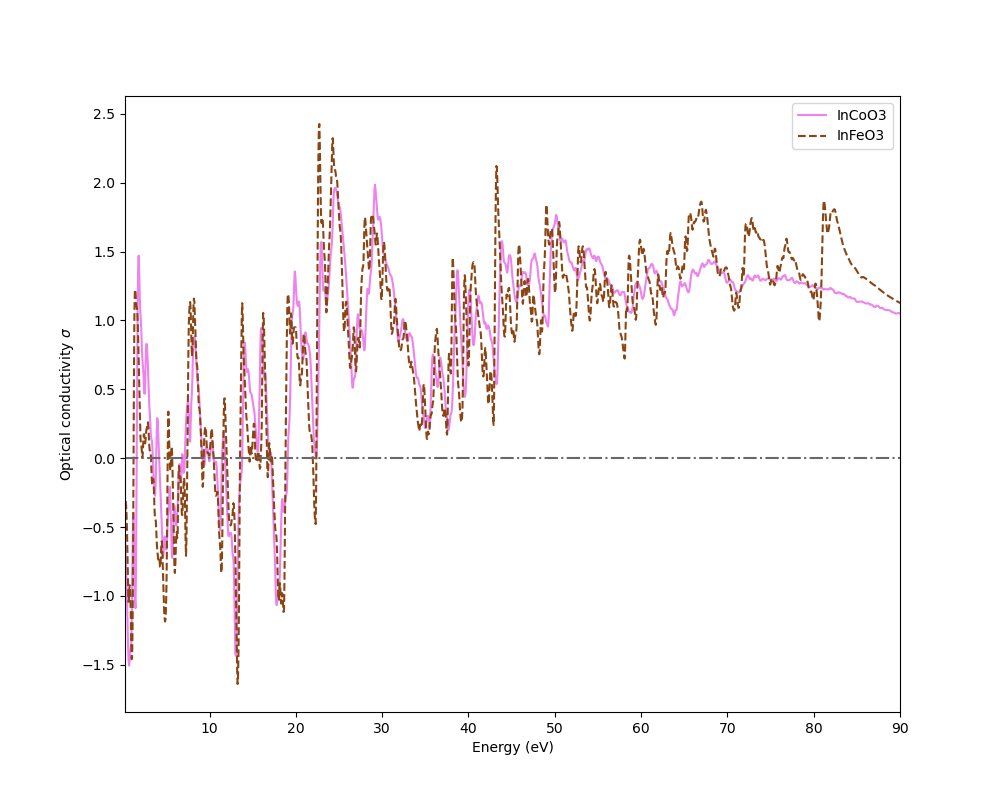
\includegraphics[width=\textwidth]{opcondimagev}
    \end{adjustbox}
    The optical conductivity of a material specifies the electric 
    conductivity of a photon from electromagnetic absorption. Fig 6 shows the dielectric constants of InCoO3 and InFeO3. Fig 7 shows us optical conductivity between
    InCoO3 and InFeO3. Fig. 9 and 10 shows Extiction and Energuloss spectrum of InCoO3
    and InFeO3 graph respectively.

    \begin{adjustbox}{center,caption={Extiction graph of INCoO3 and InFeO3},label={somelabel},nofloat=figure,}
        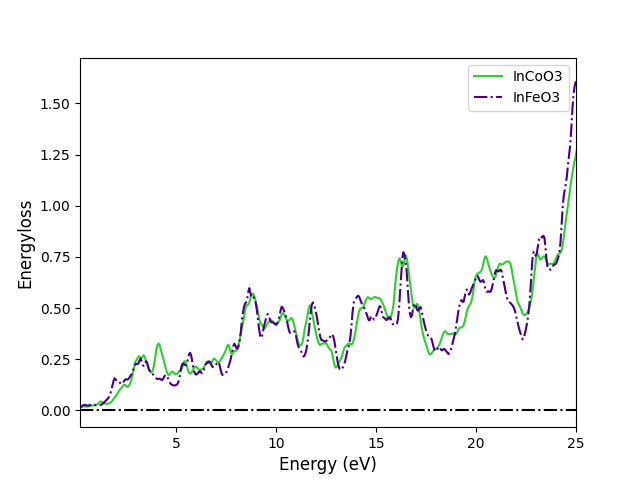
\includegraphics[width=\textwidth]{ex}
    \end{adjustbox}
    

    \begin{adjustbox}{center,caption={Energyloss spectrum of InCoO3 and InFeO3},label={somelabel},nofloat=figure,}
        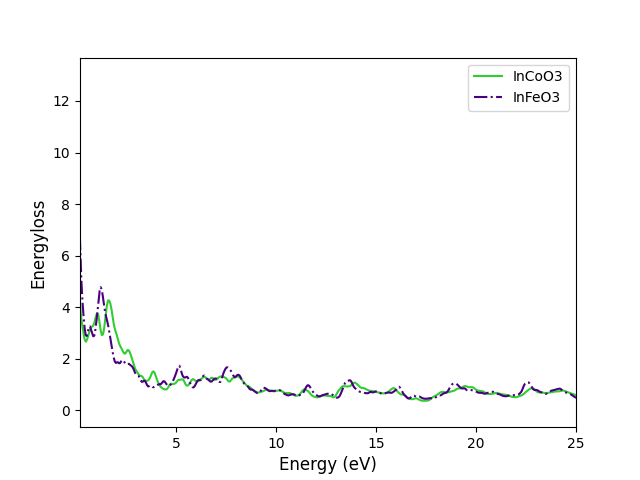
\includegraphics[width=\textwidth]{enloss}
    \end{adjustbox}

    \section{Conclusion}
    We performed a study on  InCoO3 and InFeO3\cite{r2} perovskite cubic materials using  DFT simulations for their structural, optical, and dielectric properties. InCoO3
    and InFeO3 structures show identical indirect bandgap while InFeo3 shows more magnetic than InCoO3. Fe is a better contender than Co for optical absorption 
    and optical conductivity. Both the material can be an excellent choice for various photovoltaic applications, memory devices, and more. InCoO3 give band-gap Of
    0.0017eV and InFeO3 give band-gap of 0.0034eV. So, they are magnetic materials.
    
    
    \bibliographystyle{plain}
    \bibliography{ref.bib}
\end{document}